\chapter{Methods}
\label{chapter4}
This chapter discusses the methods and approaches implemented for each part of the shopkeeper project, along with the data and testing information. I have tried to include reports of changes and limitations of each feature where appropriate
\section{The Bowl}
The bowl is a container Baxter uses to store his sweets in. The eventual aim of using the bowl was for Baxter to be able to recognise it on the table, scoop some sweets out and move on to giving them to the customer.
\subsection{Recognition}
The first thing Baxter needed to do in his shop is to be able to recognise the bowl. This section shows how Baxter uses the Kinect to find the bowl on the table, identifying it from a range of other objects. The Kinect produces a pointcloud, a set of 3D points in the Kinect's coordinates system. The first task to do when recognising the bowl, was to pick a type of bowl that would be easily visible in the pointcloud. Multiple bowl types were trialled, until it was decided white polystyrene bowls would be a good overall choice. This is because, unlike other bowls, the rim was always clearly visible in the cloud and polystyrene is an easy material to grab and manipulate. Plastic and foil materials were too reflective to show up constantly.
\subsubsection{Segmentation and Recognition}
To recognise the bowl on the table, the vision system first separates objects from the table, then separates those points into individual clusters. To eliminate noise, a colour segmentation is performed to find only the white objects on the table. The bowl can then be found by looking for the rim as a circle in 3D space. The overall process is carried out by multiple algorithms, shown in the images and explained below.
\newline\newline
\textbf{1. Tabletop Object Detection/Segmentation} - 
This method works by detecting the table in the pointcloud by finding the dominant plane using RANSAC. Points above this plane are then considered to be objects on top of the table, which are then segmented from the points that belong to the table. This results in a pointcloud without any interference from the table. \textbf{\Cref{fig:objectcluster}} shows an example of the processed pointcloud with the bowl and sweets separated from the points on the table. This separation from the tabletop was developed using the \textit{pr2\_object\_manipulator} ROS package, located and explained here\footnote{Tabletop object detector documentation. \url{http://wiki.ros.org/tabletop_object_detector}}.
\begin{figure}[H]
    \centering
    \begin{subfigure}[b]{0.475\textwidth}
        \centering
        \caption{}
        \label{fig:objectcluster}
        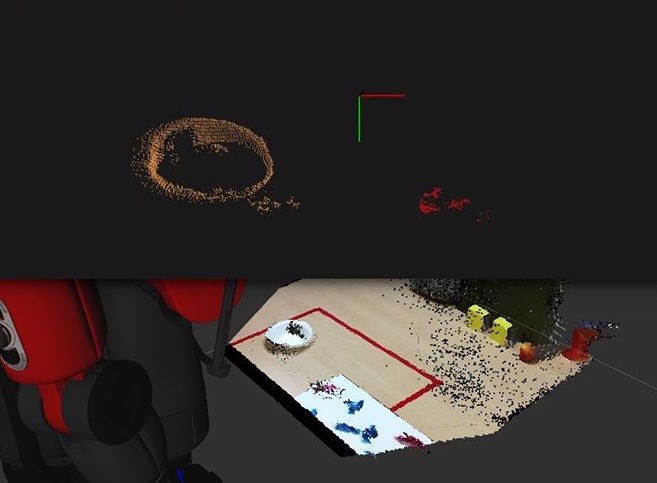
\includegraphics[width=\textwidth, height=5cm]{regiongrowing.jpg}
    \end{subfigure}
    \hfill
    \begin{subfigure}[b]{0.475\textwidth}  
        \centering 
        \caption{}
        \label{fig:whitebowl}
        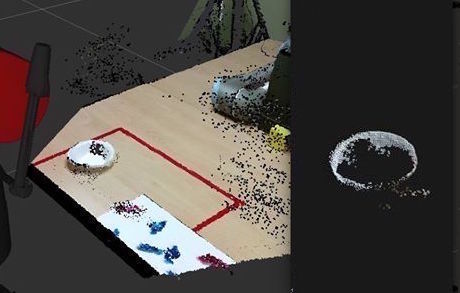
\includegraphics[width=\textwidth, height=5cm]{whitecloud.jpg}
    \end{subfigure}
    \begin{subfigure}[b]{0.475\textwidth}   
        \centering 
        \caption{}
        \label{fig:bowlcircle}
        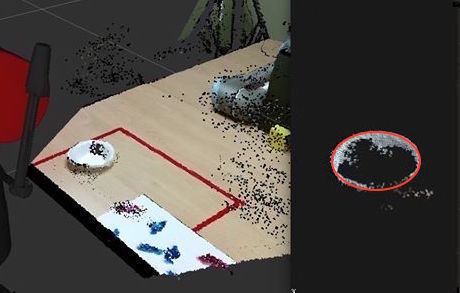
\includegraphics[width=\textwidth, height=5cm]{circlecloud.png}
    \end{subfigure}
    \quad
    \begin{subfigure}[b]{0.475\textwidth}   
        \centering 
        \caption{}
        \label{fig:rvizbowl}
        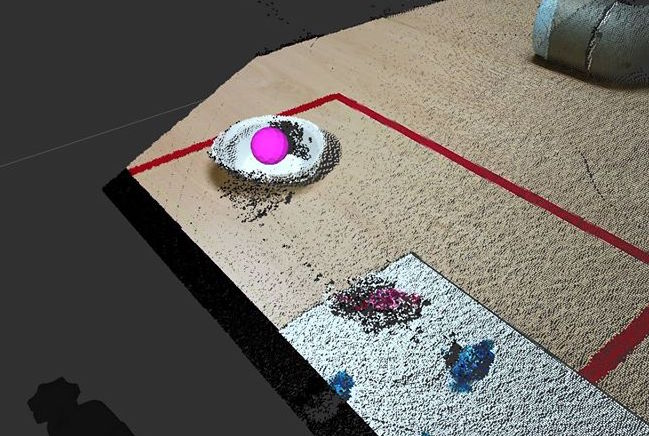
\includegraphics[width=\textwidth, height=5cm]{bowlcentre.jpg}
    \end{subfigure}
    \caption{Overall bowl recognition process. Each of the images has a view of the processed pointcloud and a view of the actual cloud from the Kinect in RViz. (a) Object clustering in the pointcloud. (b) RGB colour segmentation. (c) 3D circle detection using RANSAC. (d) Visualization of the bowl centre in RViz.}
\end{figure}
\textbf{2. Object Clustering} - 
The purpose of this algorithm is to separate the points in the pointcloud into clusters, ones which are close enough to represent the individual objects on the table. The theory behind this algorithm is it takes in the indices and estimated normals of the pointcloud and for each possible region, calculates a K-nearest neighbour search over the indices. During this search, it compares each point with another, checking first for a specified smoothness constraint, then if the deviation between normals is within a specified angle. If that is satisfied, then the difference in curvature is tested, allocating the points to the appropriately separated clusters. This algorithm uses the region growing segmentation implementation located in the PCL ROS package\footnote{Region growing segmentation documentation. \url{http://pointclouds.org/documentation/tutorials/region_growing_segmentation.php}}. Whilst using this algorithm, different values were tested. Variables such as number of neighbours, smoothness and curvature constraints were tested until the resulting cloud produced reliably clustered objects. In \textbf{\Cref{fig:objectcluster}}, you can see the points representing the bowl have been separated into one cluster and the sweets into another.
\newline\newline
\textbf{3. Colour-Based Segmentation} - 
Whilst testing the bowl detection methods, it became clear that with the Kinect, there were clear noise issues caused by certain objects in the Kinect's view. Baxter's arms especially caused severe black noise to appear around them, making it harder to segment the bowl out from other objects. Therefore, a colour segmentation method was used to separate the white bowl from the interfering black and other coloured clusters. This algorithm was written myself as the PCL library didn't provide a good solution for this method. This was done by looping over the points in each cluster and averaging the RGB values of each one. Then, only the clusters with a high enough R, G and B threshold were used, so that the resulting pointcloud contained only the points for the bowl and any other white object on the table. This method could be expanded to recognise other coloured bowls relatively easily, by finding the correct thresholds for other colours. \textbf{\Cref{fig:whitebowl}} shows the white segmented pointcloud with no black points/noise.
\newline\newline
\textbf{4. Detection of the Bowl Rim} - 
The most significant part of the bowl that tended to show up in the Pointcloud was the bowl's rim. From that information, it was decided that the simplest solution was to find the rim by searching for a specific sized circle within a plane of the 3D pointcloud. This method was implemented by using the RANSAC algorithm to detect the points that best fit a circle shape within any particular plane. This method in the PCL library is especially good at allowing variation in it's detection\footnote{RANSAC model example. \url{http://docs.pointclouds.org/trunk/group_sample_consensus.html}}. By varying distance thresholds and minimum/maximum circle radius values, the bowl was found successfully, even with gaps in the rim (which could occur when Baxter's hands went in front of the bowl). The successful rim detection is shown in \textbf{\Cref{fig:bowlcircle}}. After the circle model had been found in the white Pointcloud, the x, y and z centre coordinate of the bowl's rim was then known in the Kinect's frame coordinates.
\newline\newline
\textbf{5. Averaging and Transformations} - 
After the bowl was found in the Kinect's frame, when publishing in RViz, it was clear  whilst the centre point was always within the bowl, it wasn't a reliably constant bowl centre. Therefore, a new ROS node was created that took in the previous result, averaged the centre value over 20 frames and then outputted a new averaged centre point. This point was a lot more stable for Baxter to use. After, using the averaged bowl centre, that point was transformed into Baxter's torso frame and published, so the values could be used for bowl manipulation. To make sure the correct centre of the bowl was detected, it was visualised in RViz, shown in \textbf{\Cref{fig:rvizbowl}}.
\newline\newline
\textbf{Improvements} - 
The basic approach to recognising the bowl is described above. However, as the system began more rigorous testing, when the basic shop system was being put together, the detection was not accurate enough for Baxter to always be able to grip the edge of the bowl. Therefore, a few improvements and changes were added to the system.
\newline\newline
Due to increased noise in the Kinect's Pointcloud recordings, the averaging over 20 frames was not reliable enough to keep a fixed centre. To counteract this, a cumulative average was taken instead, meaning that if there was interference, the recognised bowl centre would not be affected as much. Another improvement was to reduce noise at the segmentation stage. To do this, a larger minimum clustering size was used when clustering the objects, so less areas of noise were included in the bowl rim detection. This resulted in a stable centre for the bowl in multiple positions on the table, as shown in the testing below.
\subsubsection{Testing}
To determine whether the recognition was reliable enough, multiple tests were taken for the bowl recognition and noted down in a spreadsheet, found in the Github repository\footnote{Github repository: Bowl Recognition Tests. \url{https://github.com/um10kh/baxter-project/blob/master/Trials/Bowl\%20Recognition\%20Tests.xlsx}}. The main method of testing whether the bowl recognition was accurate enough was devised by getting Baxter to grab the edge of the bowl using the bowl's centre coordinate found through the vision system. Since grasping the bowl is a key aspect in retrieving sweets from the bowl, it made sense that the recognition system would have to be accurate enough for Baxter to be able to reliably repeat this feat.
\captionsetup[figure]{justification=centering}
\begin{figure}[H]
        \centering 
        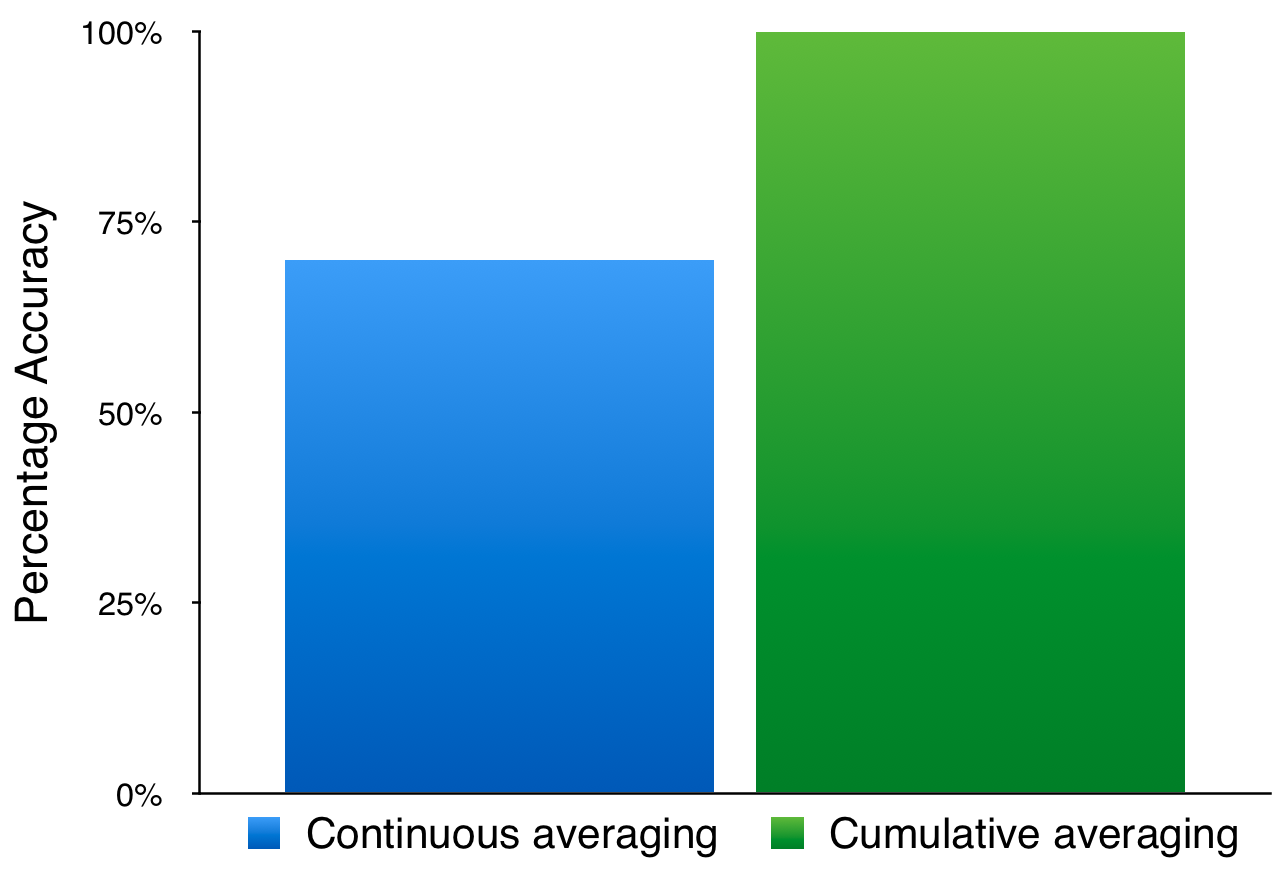
\includegraphics[width=0.475\textwidth, height=5cm]{bowlrecognition.png}
        \caption{Comparison of repeated grasps using different techniques over time.}
        \label{fig:bowlRecognition}
\end{figure}
\vspace{-0.2cm}For the initial rolling average over 20 frames and the cumulative averaging methods (mentioned in the sections above), Baxter was tasked with grasping the edge of the bowl 10 times with each method. The efficiency was then calculated as a percentage of the bowl grasping accuracy, shown above in \textbf{\Cref{fig:bowlRecognition}}. As you can see, the cumulative averaging obtained a 100\% accuracy over 10 tests and therefore seemed the more reliable and sensible choice to use in the overall system. The only issue with the cumulative average method is after the bowl has been moved, if the bowl had previously been in place for a long time, the centre will end up being a mixture between the two positions. Therefore, a reset option had to be implemented so that when Baxter moved the bowl, a new cumulative average was taken when looking for the moved bowl.
\newline\newline
\textbf{Limitations}\newline
Limitations on the bowl recognition system seemed to be based around common recognition issues within computer vision. The rim detection could get confused if two light-coloured, round-shaped objects were on the table, meaning that in object clutter, the cumulative, detected centre of the bowl would be offset by other, falsely recognised `bowl rims'. Solutions to this limitation would be complex and would possibly need a 3D model built using the bowl so that Baxter could accurately recognise and distinguish it from other objects. Issues also occurred when Baxter's hand obscured the bowl significantly, preventing the bowl's circular rim from being detected. The simple way to get around this limitation was to only check where the bowl's location was when the system knew Baxter's arm was out of the way.
\subsection{Manipulation}
With the bowl having been recognised, the next step was for Baxter to retrieve sweets from the bowl so he could separate them out on the table. Two main methods for this were trialled, first scooping methods were tested, trying different ways for Baxter to scoop out sweets with his grippers. Secondly, Baxter tipped the bowl onto the table at different angles to get the sweets out. Both methods are explained in more detail here:
\subsubsection{Scooping Methods}
Firstly, several methods of scooping were trialled for Baxter to scoop sweets out of the bowl with his gripper. These methods were developed through theories and trials and then tested to see which methods were the most efficient.  Different variables to consider were things like gripper distance - the distance between the grippers when closed, angle of entry to the bowl and gripper movement before grasping. Testing for the reliability of these methods are shown in the \hyperref[sssec:ScoopTest]{\textbf{Scooping Tests}} section and videos on all of the different scooping methods are located on the Github repository\footnote{Github repository: Videos - Bowl Scooping Methods. \url{https://github.com/um10kh/baxter-project/tree/master/videos/Bowl\%20Scooping\%20Methods}}.
\newline\newline
\textbf{Grasp from Above} - The grasp from above method was the simplest, first approach taken, where Baxter retrieves the centre of the bowl, goes slightly above it at a fixed height, then moves slowly down into the bowl and closes his gripper. \textbf{\Cref{fig:graspfromabove}} shows this grasping method in action. To an extent, this method was one of the best at gripping individual sweets from a full bowl however, the problem was the approach. During this method, Baxter would try and go to a fixed depth and then grab sweets. Unfortunately, without analysing the sweet's orientation in the bowl first, the end of Baxter's grippers would get caught on them before reaching the specified depth. Then the sweets underneath the grippers would be crushed, which was seen as a problem for a shopkeeper. 
\begin{figure}[H]
    \centering
    \begin{subfigure}[b]{0.475\textwidth}
        \centering
        \caption{}
        \label{fig:graspfromabove}
        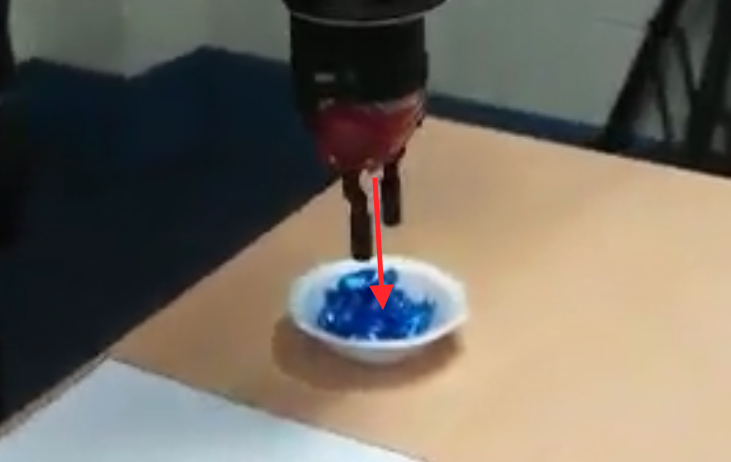
\includegraphics[width=\textwidth, height=5cm]{graspfromabove.png}
    \end{subfigure}
    \hfill
    \begin{subfigure}[b]{0.475\textwidth}  
        \centering 
        \caption{}
        \label{fig:graspandshake}
        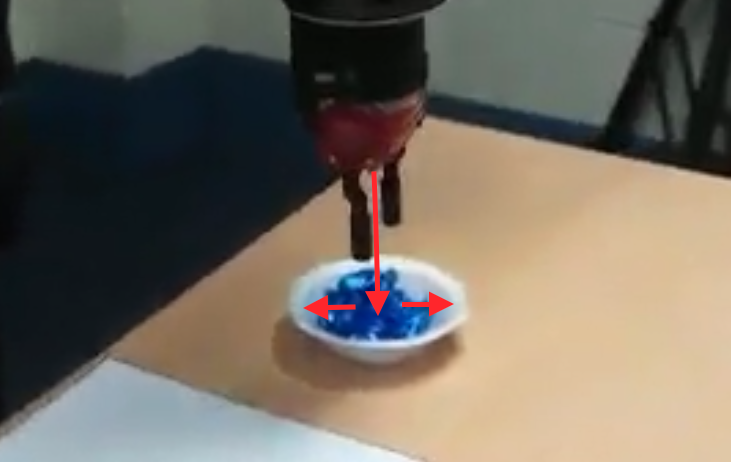
\includegraphics[width=\textwidth, height=5cm]{graspandshake.png}
    \end{subfigure}
    \caption{Grasping methods: (a) Grasp from above. (b) Grasp and shake}
    \vspace{0.2cm}
\end{figure}
\textbf{Grasp and Shake} - A second version of the grasp from above method used a slightly adapted method of bowl entry, where Baxter went near the rim, then lowered his hand moving from side to side. The basic idea of this grasp is shown in \textbf{\Cref{fig:graspandshake}}. In theory, that would reduce the likelihood of hitting and crushing sweets on the way into the bowl as the hand would be able to shake itself in. However, yet again, if the grippers approached on top of some sweets, they would be crushed and then moved from side to side, staying stuck. Another fault of this method came from trying to empty the bowl. Due to the position being approached at the centre, only sweets in the centre could be retrieved, pushing other sweets to the side of the bowl. That spawned the idea for creating a scooping method that tilted the bowl in future trials.
\newline\newline
\textbf{Scoop from the Side} - This method worked very much how it sounds, using Baxter's gripper to approach the bowl at an angle to try and scoop some sweets up. \textbf{\Cref{fig:scoopfromside}} shows a diagram of this method. The downside to this approach came apparent after multiple trials, where Baxter ended up pushing sweets to one side of the bowl so on repeated attempts, it could no longer reach them. This method did however improve Baxter's ability not to crush sweets, as the angled entry meant he was less likely to get stuck on a sweet, as he could just push it to one side. Due to the sweets being pushed aside, the idea of tilting the bowl again was theorised to be able to retrieve more sweets from the bowl over time.
\begin{figure}[H]
    \begin{subfigure}[b]{0.475\textwidth}   
        \centering 
        \caption{}
        \label{fig:scoopfromside}
        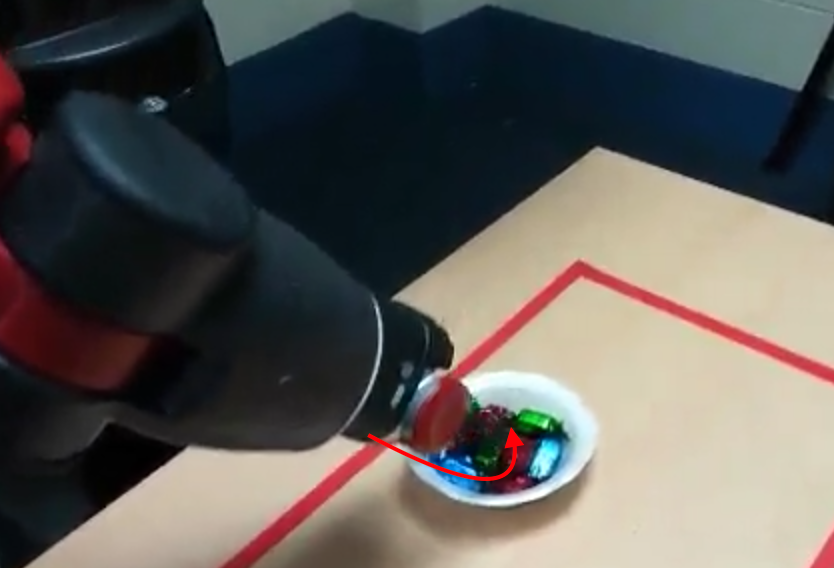
\includegraphics[width=\textwidth, height=5cm]{scoopfromside.png}
    \end{subfigure}
    \quad
    \begin{subfigure}[b]{0.475\textwidth}   
        \centering 
        \caption{}
        \label{fig:tiltandshake}
        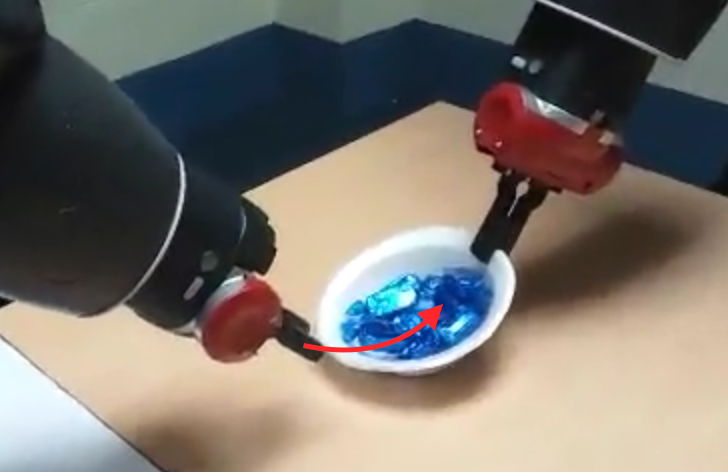
\includegraphics[width=\textwidth, height=5cm]{tiltandshake.png}
    \end{subfigure}
    \caption{Grasping methods: (a) Scoop from the side. (b) Tilt and scoop.}
\end{figure}
\textbf{Tilt and Scoop} - This method came by combining ideas from the previous methods to develop a more reliable method of scooping sweets. Firstly the left hand would grip the side of the bowl and tilt it so sweets fall down to one side, then the right hand gripper would come in and try and scoop some sweets up. \textbf{\Cref{fig:tiltandshake}} shows this grasping method in action. This process, while reliable on tilting the sweets, was unreliable on it's consistency, as the approach sometimes managed to pick up one or two sweets, but most often it missed them on a random approach.
\subsubsection{Scooping Tests}
\label{sssec:ScoopTest}
In the Github repository\footnote{Github repository: Grasping Methods Tests. \url{https://github.com/um10kh/baxter-project/blob/master/Trials/Grasping\%20Methods\%20Tests.xlsx}}, there is a spreadsheet showing trials of each type of scooping method mentioned above. For each method, there was a trial regarding it's efficiency from grasping sweets from a full bowl (the less grasps Baxter could get the customer's sweets in the better) and repeated trials were carried out, to see how well they performed over time after the initial scoops.
\newline\newline
In \textbf{\Cref{fig:timegrasp}}, the y axis shows the number of sweets grasped and the x axis shows the current grasp attempt number. The graph shows the tilt and scoop method was the most reliable grasping method over time. This suggested that the tilting was beneficial and meant it prevented sweets from being pushed to one side after initial grasps. The problem with all methods in this figure however, is that sweets were not grasped particularly efficiently. There was a maximum of around 3 sweets retrieved after 8 attempts, meaning the customer would have to wait a very long time if they wanted 3 or more sweets (which ideally would be possible).
\begin{figure}[H]
    \captionsetup[subfigure]{justification=centering}
    \begin{subfigure}[b]{0.475\textwidth}   
        \centering 
        \caption{}
        \label{fig:timegrasp}
        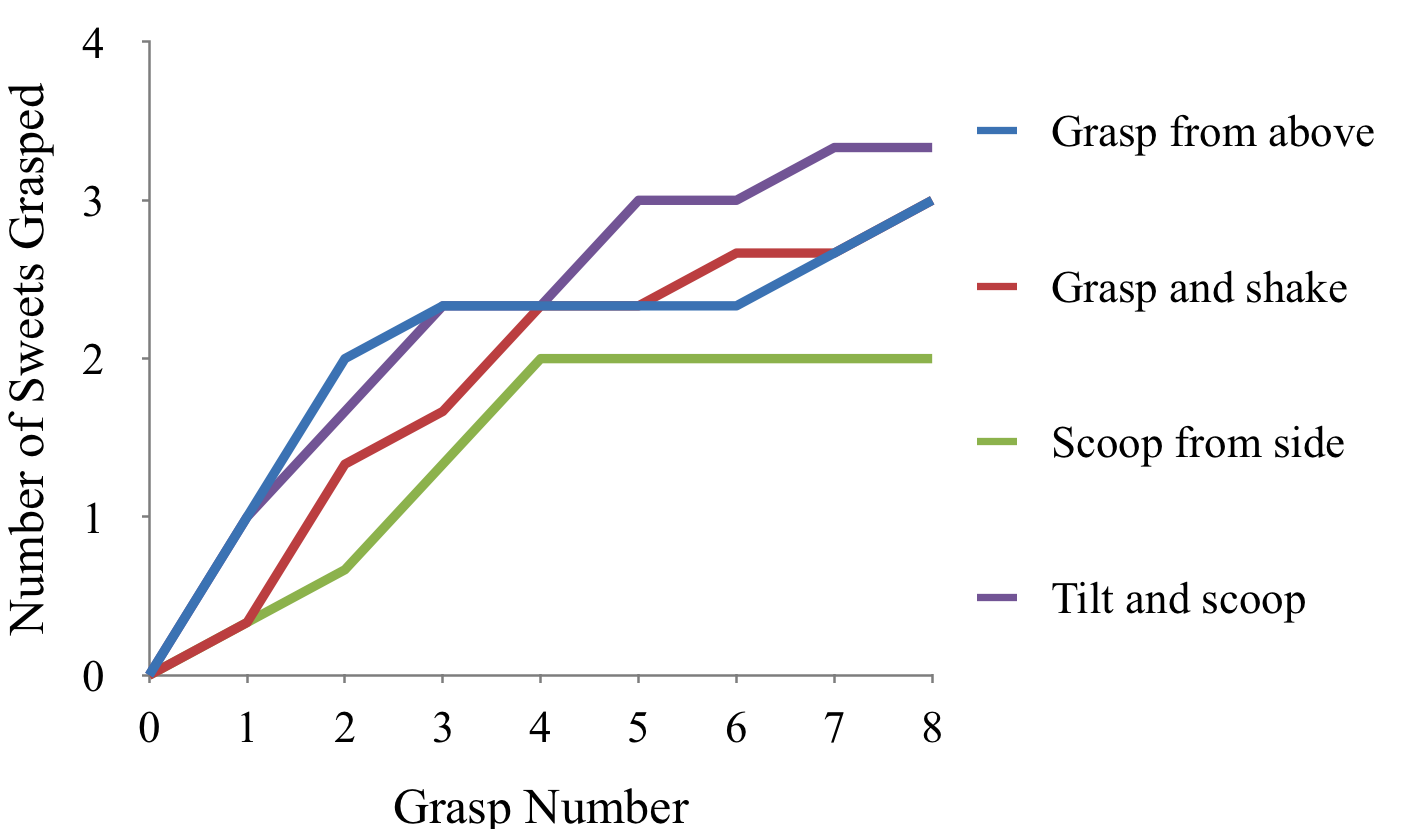
\includegraphics[width=\textwidth, height=5cm]{graspovertime.png}
    \end{subfigure}
    \begin{subfigure}[b]{0.475\textwidth}   
        \centering 
        \caption{}
        \label{fig:averagegrasp}
        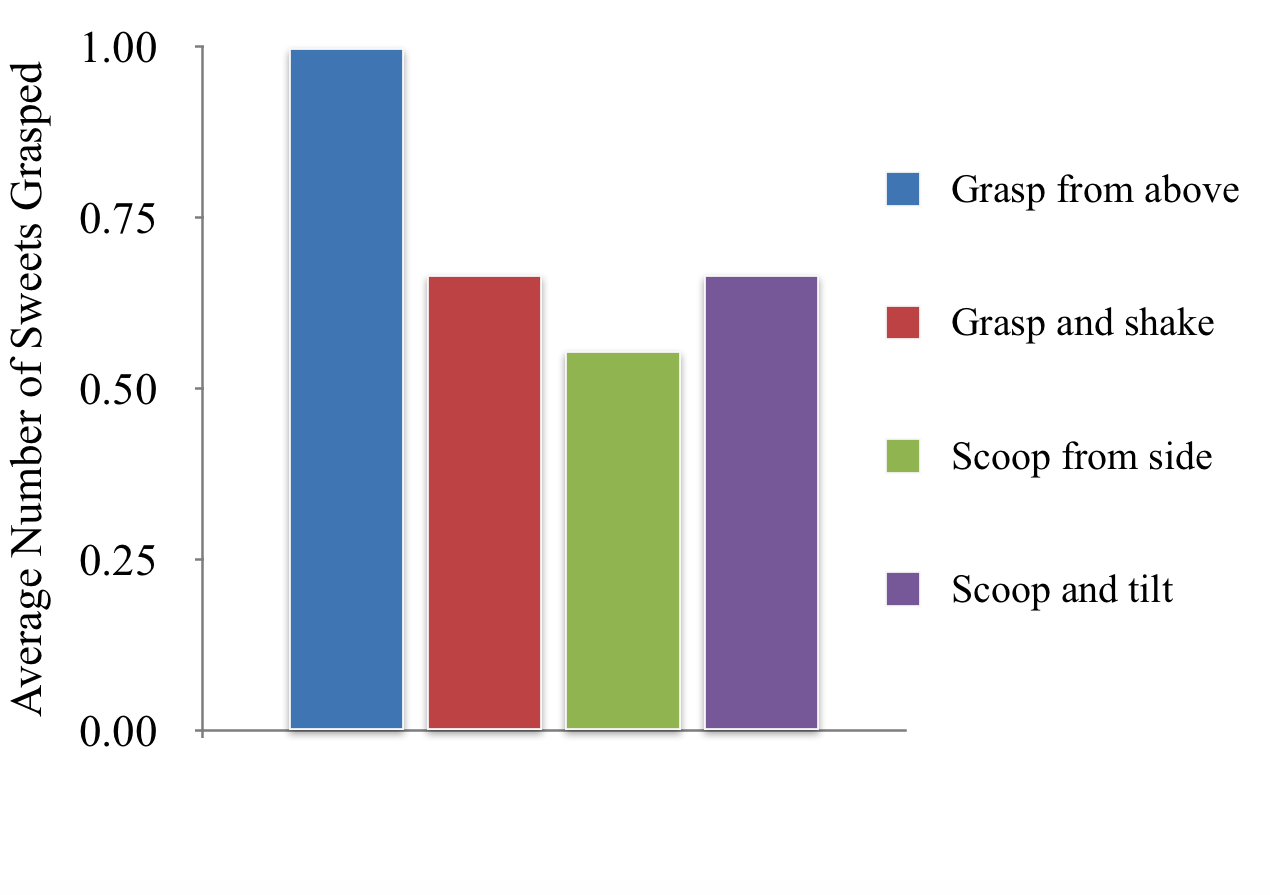
\includegraphics[width=\textwidth, height=5cm]{averagegrasp.png}
    \end{subfigure}
    \caption{Scooping test graphs: (a) Comparison of repeated grasps using different techniques over time. (b) Comparison of the average sweet number grabbed from a full bowl.}
\end{figure}In \textbf{\Cref{fig:averagegrasp}} you can see that, on average, from a full bowl of sweets, the grasp from above method was the most effective, averaging one sweet grasped over ten attempts. The main thing to point out here was that the maximum average grasped from a full bowl was only one sweet. In a shop-like scenario, a customer will most likely want more than one sweet, so if Baxter had to grasp one at a time, the process would take a very long time. After testing these grasping methods, it was determined that no one scooping method would be efficient enough for Baxter to use. This was due to the reliability of these methods not being sufficient enough for Baxter to grab multiple sweets at a time. By taking inspiration from the tilt and scoop method, it was decided that tipping sweets from the bowl onto an area on the table would be a possible solution to get more sweets in a shorter number of attempts. This was trialled in the  \hyperref[sssec:tippingmethods]{\textbf{next section}}.
\subsubsection{Tipping Methods}
\label{sssec:tippingmethods}
After deciding scooping the sweets was not a reliable enough method, some bowl tipping methods were trialled to attempt to achieve a better efficiency. Each method was again developed through manipulation trials. In each trial, the sweets were attempted to be tipped and dropped onto a rectangular area designated for sweet singulation. This brought in several new factors to consider such as whether the sweets landed successfully in the area, how many sweets fell next to each other (the more often that happened the harder for Baxter to separate them later) and where in the area should the sweets be tipped.
\newline\newline
Different variables considered in these methods included factors such as tipping height, tipping angle, tipping location and tipping speed. Tipping added another issue to the manipulation because once sweets had been tipped out of the bowl, it was harder to get the remaining ones out, meaning an incremental approach had to be taken, increasing angles and speed to retrieve them. Testing for the tipping methods are shown in the \hyperref[sssec:TippingTest]{\textbf{Tipping Tests}} section and videos of the methods are located on the Github repository\footnote{Github repository: Videos - Bowl Tilting Methods. \url{https://github.com/um10kh/baxter-project/tree/master/videos/Bowl\%20Tilting\%20Methods}}.
\begin{figure}[H]
    \captionsetup[subfigure]{justification=centering}
    \begin{subfigure}[H]{0.475\textwidth}   
        \centering 
        \caption{}
        \label{fig:verticaltilt}
        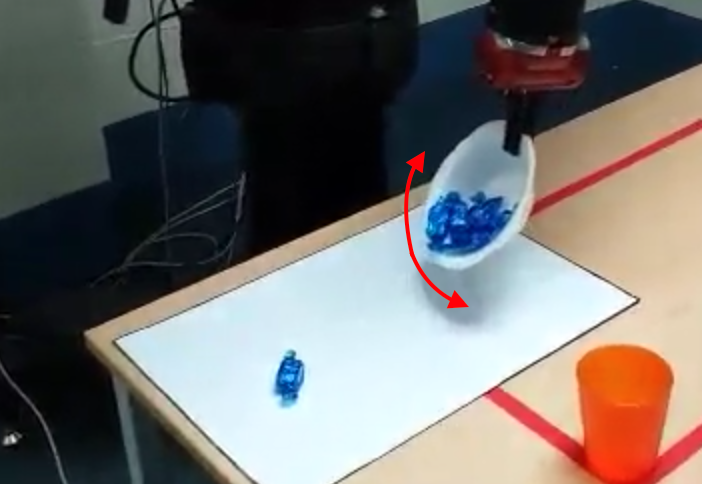
\includegraphics[width=\textwidth, height=5cm]{verticaltilt.png}
    \end{subfigure}
    \begin{subfigure}[H]{0.475\textwidth}   
        \centering 
        \caption{}
        \label{fig:horizontaltilt}
        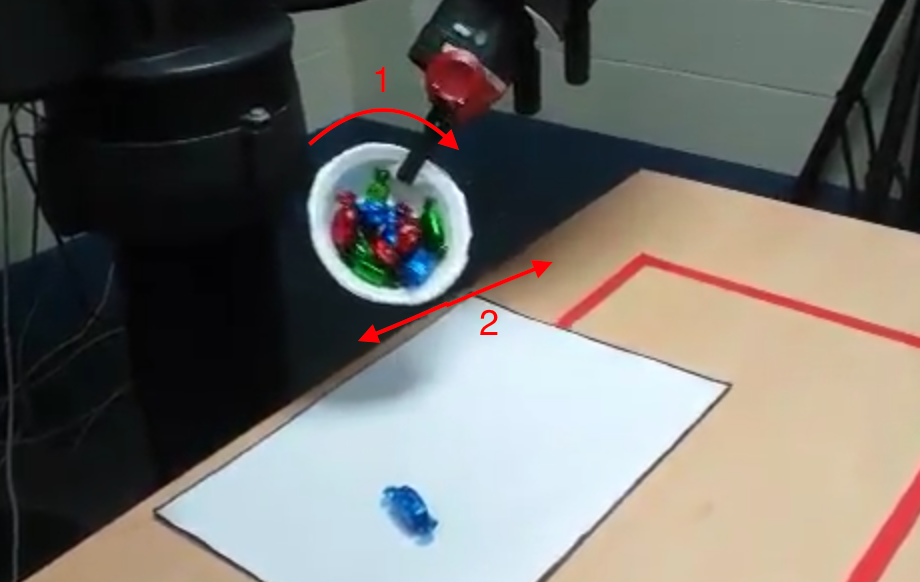
\includegraphics[width=\textwidth, height=5cm]{horizontaltilt.png}
    \end{subfigure}
    \caption{Tipping methods: (a) Vertical tilt. (b) Horizontal tilt.}
\end{figure}
\textbf{Vertical Tilt} - 
A vertical tilting method was the first tipping method trialled, where Baxter would grasp the bowl from the side, then raise the `elbow' of his arm so that the bowl was tilted at an angle. Then Baxter would rotate up and down, shaking the sweets out of the bowl onto the table,  as shown in \textbf{\Cref{fig:verticaltilt}}. The optimal number found through testing was for Baxter to tip the sweets out once in the centre-right of the sweet area and once in the centre-left so there was a reasonably even spread of sweets tipped out on both sides of the area. This method caused issues in reliability over multiple tilts. Sometimes, when there were sweets down in the bottom of the bowl, no matter how high the tilt angle was, they were hard to shake out without completely tipping the bowl upside down. The horizontal tilt method was developed from the flaws in this method, in theory to gain some extra control over the tilting angle by using Baxter's gripper rotation instead of the `elbow' rotation.
\newline\newline
\textbf{Horizontal Tilt} - This method was similar to the vertical tilt as mentioned above but instead, Baxter tilts the bowl using his gripper so there was more control over the tipping. Another factor added to this method was that instead of shaking the bowl up and down, Baxter instead shook it in a upward diagonal motion, shaking sweets upwards and out of the bowl at the same time, shown in \textbf{\Cref{fig:horizontaltilt}}. Whilst this technique added a worry of throwing sweets too far out of the bowl, it did help get the sweets towards the bottom of the bowl. The efficacy of this method against the vertical tilt is discussed in the testing below.
\subsubsection{Tipping Tests}
\label{sssec:TippingTest}
To test the tilting methods, a similar approach was taken to the bowl grasping tests. In these tests, two different versions of the horizontal and vertical tilts were observed. The 1st iteration of these tilts had a smaller tilting angle and a smaller shaking height and the 2nd iterations had higher values for these. Each of these methods were judged on their ability to tip sweets onto the page from a full bowl and their ability to separate the sweets on the table to be easily graspable.
\begin{figure}[H]
    \captionsetup[subfigure]{justification=centering}
    \begin{subfigure}[H]{0.475\textwidth}   
        \centering 
        \caption{}
        \label{fig:avsweetstipped}
        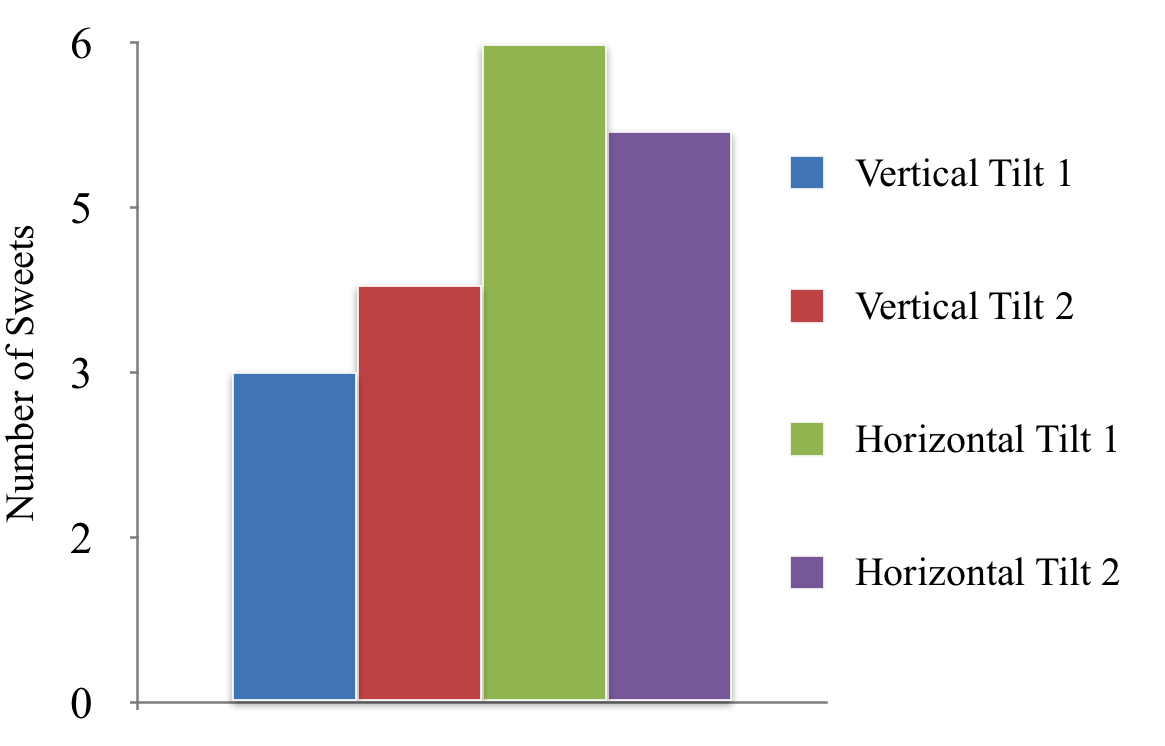
\includegraphics[width=\textwidth, height=5cm]{averagesweetstipped.png}
    \end{subfigure}
    \begin{subfigure}[H]{0.475\textwidth}   
        \centering 
        \caption{}
        \label{fig:percentageseparated}
        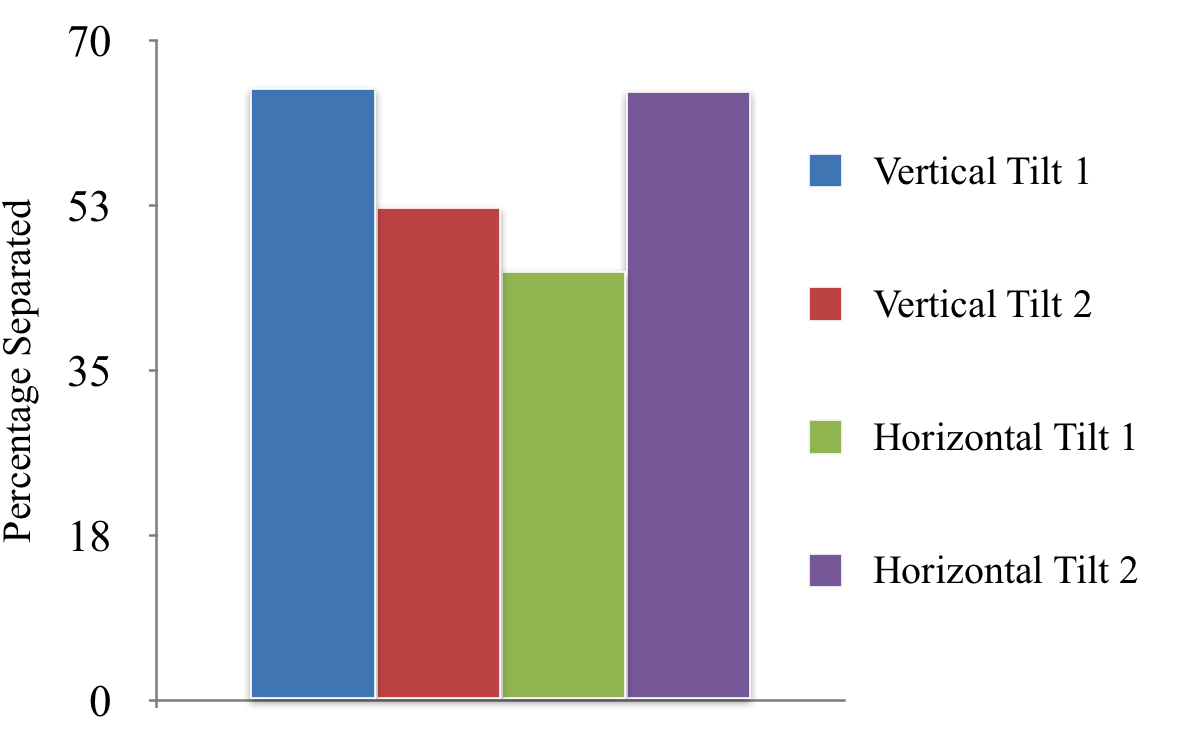
\includegraphics[width=\textwidth, height=5cm]{separatedsweets.png}
    \end{subfigure}
    \vspace{-0.2cm}
    \caption{Tipping methods graphs: (a) Average number of sweets tipped onto the table. (b) Percentage of sweets separated on the table by each method.}
\end{figure}
As you can see from \textbf{\Cref{fig:avsweetstipped}}, the horizontal tilting methods tipped more sweets onto the table in one tilt over the vertical tilting methods. By looking at \textbf{\Cref{fig:percentageseparated}}, the percentage sweets separated was highest using Horizontal Tilt 2 and Vertical Tilt 1. By combining the best results from both tests, it was decided that the second horizontal tilting method would produce the most desirable results for tipping and separating sweets on the table. The recorded spreadsheet for this test is located here\footnote{Github repository: Tipping Methods Tests. \url{https://github.com/um10kh/baxter-project/blob/master/Trials/Tipping\%20Methods\%20Tests.xlsx}}.
\section{The Sweets}
Once Baxter had seen the bowl and retrieved sweets from it, the next task was for Baxter to recognise the sweets and be able to individually pick the requested sweets up for a customer. This task was split into recognition, singulation and manipulation methods.
\subsection{Recognition}
The task of Baxter recognising the sweets involved him being able to look at an area of the table with sweets retrieved from the bowl on and determine how many sweets there were in that area along with what type/colour each sweet was. The problem with recognising the sweets using the Kinect was that the sweets were such small objects,  the noise in the Kinect meant a significant number of sweets weren't picked up after segmenting objects from the table. Therefore an alternative method was proposed using OpenCV. The idea behind this method was for Baxter to capture an image of the table with the sweets on using his hand camera. Then from that image, OpenCV image processing techniques could be applied to separate the sweets into individual objects, from which the shapes, centres and colours could be obtained.
\subsubsection{Sweet Background Detection}
The first task in separating the sweets was to have Baxter to only look in the area the sweets were placed on the table, so any other objects/sweets on the table would not interfere. It was decided the easiest way to segment this area out was to use a white piece of paper as the background, making it easier to segment out the rest of the image. The piece of paper used was A3 in size and had a black edge drawn on, to help detect the border of the page. Multiple vision methods were trialled to try and recognise this sweet placement area, explained below.
\begin{figure}[H]
    \captionsetup[subfigure]{justification=centering}
    \begin{subfigure}[H]{0.475\textwidth}   
        \centering 
        \caption{}
        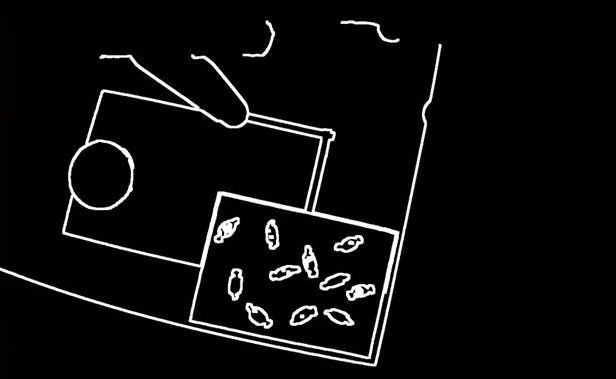
\includegraphics[width=\textwidth, height=5cm]{cannedge.jpg}
        \label{fig:edgeImage}
    \end{subfigure}
    \begin{subfigure}[H]{0.475\textwidth}   
        \centering 
        \caption{}
        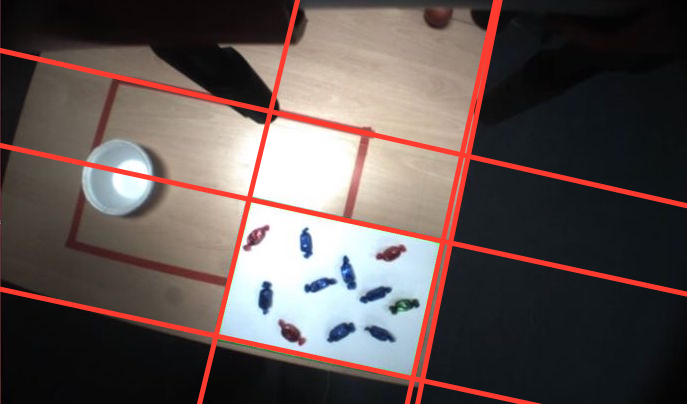
\includegraphics[width=\textwidth, height=5cm]{houghline.png}
        \label{fig:houghline}
    \end{subfigure}
    \vspace{-0.5cm}
    \caption{Sweet background detection techniques: (a) An example of Gaussian blurring, Canny Edge detection, then image opening. (b) Hough line transform used to detect the edges of the sweet area.}
\end{figure}
\textbf{Image Pre-processing} - 
Before the image from the camera could first be used, some pre-processing was taken place to reduce noise and make it easier to detect the area on the table. A Gaussian Blur was performed with a small kernel to firstly blur the image to reduce possible noise. Then, Canny Edge Detection was used to detect edges within the image, along with dilation and erosion to close any incomplete edges, resulting in a reasonably successful edge detection for the entire image, shown in \textbf{\Cref{fig:edgeImage}}.
\newline\newline
\textbf{Hough Line Transform} - 
Firstly, to find a rectangle in the image, Hough Line Transform was attempted to be used to find the individual edges of the paper. This technique was somewhat successful when attempting to distinguish between the edges however, by varying and optimising the line detection threshold, it was difficult to detect all four edges of the paper consistently. Either one or two edges kept being detected then undetected or too many edges were found (shown in \textbf{\Cref{fig:houghline}}). This resulted in reliability issues finding the rectangular area, so other methods were explored.
\begin{figure}[H]
    \captionsetup[subfigure]{justification=centering}
    \begin{subfigure}[H]{0.475\textwidth}   
        \centering 
        \caption{}
        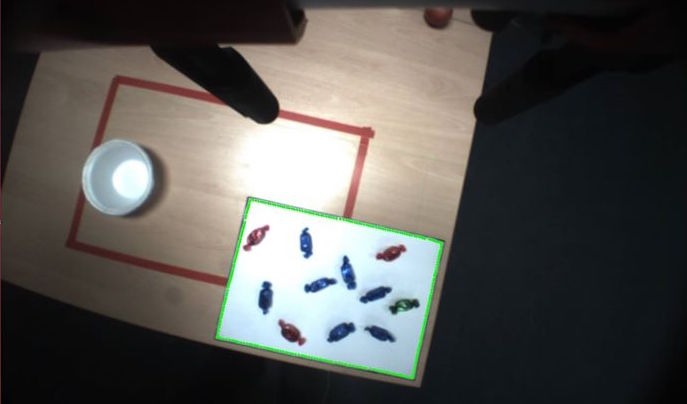
\includegraphics[width=\textwidth, height=5cm]{contourfound.jpg}
        \label{fig:greencontour}
    \end{subfigure}
    \begin{subfigure}[H]{0.475\textwidth}   
        \centering 
        \caption{}
        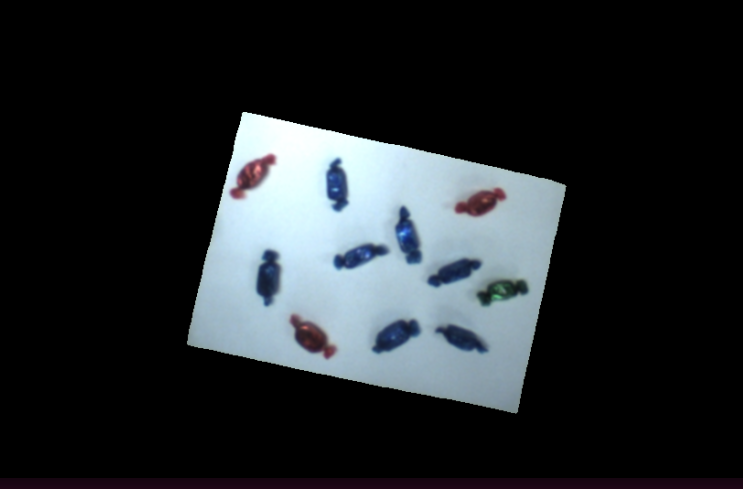
\includegraphics[width=\textwidth, height=5cm]{segmentedarea.png}
        \label{fig:sweetareamask}
    \end{subfigure}
    \vspace{-0.3cm}
    \caption{Sweet area detection using contours: (a) Green contour correctly wrapped around the sweet area. (b) Masked sweet area after contour segmentation.}
\end{figure}
\textbf{Contour Detection} - Once the black border on the area was drawn thickly enough to be consistent during canny edge detection, a contour successfully managed to wrap itself round the four edges of the paper. Due to there being many contours detected in the image, certain constraints had to be put on the detection to segment out the sweet area contour from the others. The main method of segmenting out the rectangular area then was to first eliminate the smaller contours by size (using the in-built OpenCV countourArea method) and then approximate a polygon for the countours to detect which countour was rectangular in shape. The eventual correct contour was selected and identified, shown in \textbf{\Cref{fig:greencontour}}. This contour could then produce a mask, which could segment out the rest of the image from the sweet area, shown in \textbf{\Cref{fig:sweetareamask}}, which meant that the vision system had a separated area to analyse the sweets in.
\subsubsection{Sweet Recognition}
Once the sweet placement area was reliably segmented out from the image, multiple methods were used to attempt to try and identify the individual sweets. These methods are explained below.
\newline\newline
\textbf{Hough Circle Transform}
\newline
For the simple, round sweets initially used in trials, a Hough Circle detection algorithm seemed like a sensible way to detect the simpler, round sweets. However, like the Hough Line detection used earlier, it was hard to get a constant solution, with circles being undetected throughout various received image frames (shown in \textbf{\Cref{fig:sweetcircle}}), therefore other methods needed to be tried to get a more reliable vision system.
\begin{figure}[H]
    \captionsetup[subfigure]{justification=centering}
    \begin{subfigure}[H]{0.475\textwidth}   
        \centering 
        \caption{}
        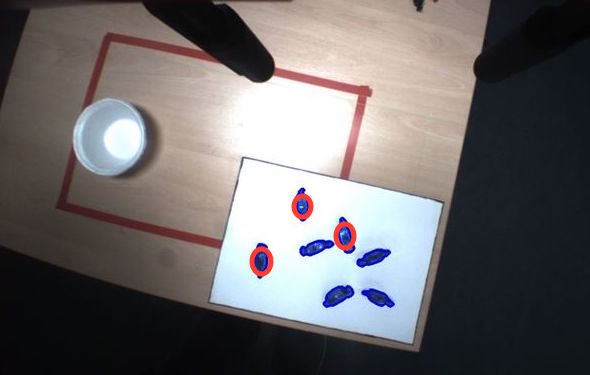
\includegraphics[width=\textwidth, height=5cm]{sweetcircle.jpg}
        \label{fig:sweetcircle}
    \end{subfigure}
    \begin{subfigure}[H]{0.475\textwidth}   
        \centering 
        \caption{}
        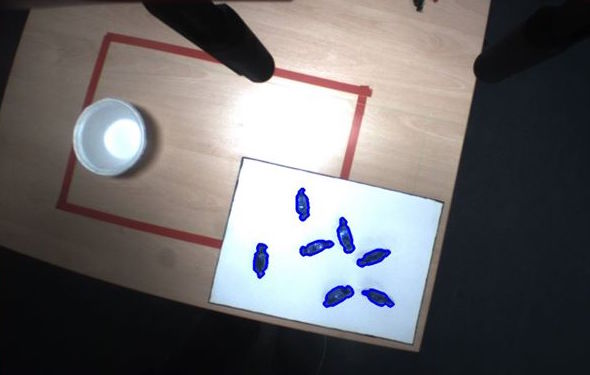
\includegraphics[width=\textwidth, height=5cm]{sweetsfound.jpg}
        \label{fig:workingblue}
    \end{subfigure}
    \vspace{-0.5cm}
    \caption{Sweet recognition techniques: (a) Sweets detected using Hough circle detection. (b) Correct blue contours found for each of the blue sweets.}
\end{figure}
\textbf{Contour Detection}
\newline
A better method was to do some image processing, Gaussian blurring, closing and opening to reliably produce a mask of a white background with some black sweets in front. The problem with using this method is due to reflections on the sweets wrappers, which caused an issue of multiple broken contours within an individual sweet, whereas a preferred method would have been to capture the whole sweet with one contour, as Baxter needs to be able to count each sweet once.
\newline\newline
\textbf{HSV Colour Segmentation with Contour Detection}
\newline
A more accurate method was found by using an existing tool called objectfinder\footnote{Github repository: Misc files - objectfinder.py. \url{https://github.com/um10kh/baxter-project/blob/master/miscFiles/objectfinder.py}}. This tool uses multiple sliders to segment an image and produce a mask using lower and upper bounds for RGB values. Since each sweet wrapper had different identifiable colours and they were placed onto a separable white background, using a range of possible HSV values could be used to identify main sweet wrapper colours - blue, green, red etc. An example of this working is shown in \textbf{\Cref{fig:workingblue}} above. The only limitation of this approach was that similar colours under light could be mixed up, for example, red and pink wrappers had overlapping HSV RGB ranges, and therefore could not be both separated and identified by this method. It did however result in very clear contours for the significantly different colours so this method was initially used for the sweet recognition. Possible improvements could have been made with shape recognition then colour analysis, which may have been able to identify a typical sweet shape and then separate by colour after.
\newline\newline
\textbf{Improvements on Colour Detection}
\newline
Whilst the HSV detection method was reasonably accurate, there were issues, which often occur in vision techniques, when the lighting changed. At different times of day, the HSV colour recognition failed, as the blue/green and green/red colourspaces overlapped in light or dark conditions. A couple of solutions were proposed as improvements on the colour detection to rectify this.
\newline\newline
\textbf{Euclidean Distance} - Since the HSV range method varied in the light, an attempt was made to capture some of the light variation. Instead of detecting a range of HSV values, an averaged HSV value was calculated using multiple samples of each colour. By analysing the mean colour of the contour multiple times for each colour, an average RGB value for red, blue and green was calculated. Then, when trying to check what colour a sweet was, the RGB value with the smallest Euclidean distance to the average  value would be the detected colour.
\newline\newline
\textbf{Neural Networks} - Neural networks are a relatively new development in AI, used to learn certain tasks by knowing the needed results, training the network to produce a set of weights to produce the desired results. Since the RGB colourspaces of the green, blue and red sweet wrappers overlapped in their values, it was decided a neural network could take some example values of the sweet's RGB values, learn them, and produce a more reliable colour recognition method.
\begin{figure}[H]
    \captionsetup[subfigure]{justification=centering}
    \begin{subfigure}[H]{0.475\textwidth}   
        \centering 
        \caption{}
        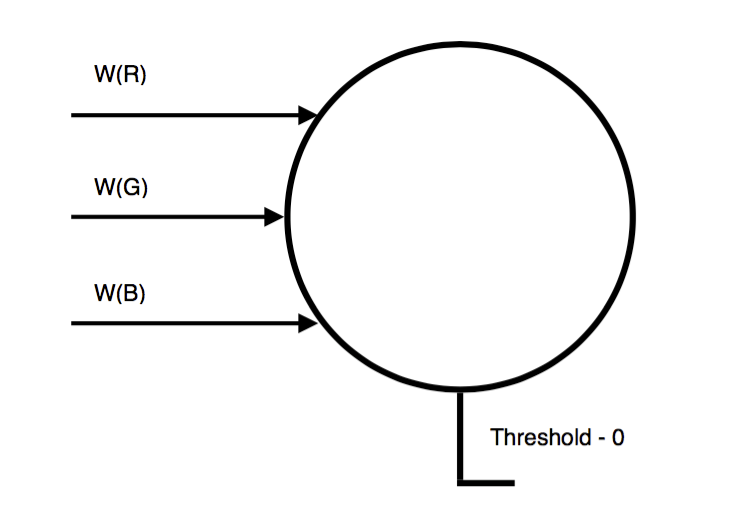
\includegraphics[width=\textwidth, height=5cm]{neural.png}
        \label{fig:perceptron}
    \end{subfigure}
    \begin{subfigure}[H]{0.475\textwidth}   
        \centering 
        \caption{}
        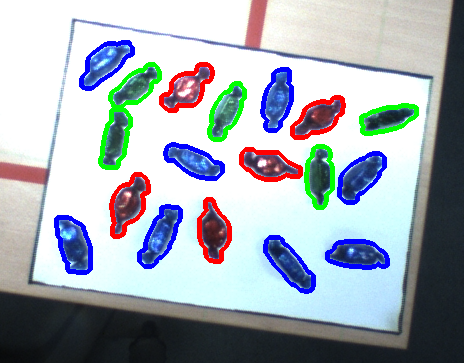
\includegraphics[width=\textwidth, height=5cm]{correctneuralimage.png}
        \label{fig:workingneural}
    \end{subfigure}
    \vspace{-0.5cm}
    \caption{Neural network images: (a) An example perceptron of the neural network with a threshold of 0. (b) An example of the correct sweet colour classification using the neural network.}
\end{figure}
This was done by first collecting a sample of 50 of each coloured sweet's RBG values. 10 images were taken of five green, red and blue sweets respectively with sweets in different positions related to the light source and at different times of day. Then the RGB values from within each sweet contour were written to a text file along with the desired result, for example: "R: 75, G: 80, B: 100, blue". This colour dataset was then used to train a simple neural network. The simple neural network design was based on the basic perceptron learning algorithm, which used a basic perceptron design, shown in \textbf{\Cref{fig:perceptron}}. More information about the basic principles of neural networks can be found here\cite{neuralnetworks}. This perceptron would ideally train using the dataset by finding four weights that would give a less than zero value if the sweet RGB values matched a colour and above zero if they didn't match. After training the perceptron weights on the dataset for each colour (ie. green vs non green values), three sets of weights were returned to classify the colours. 
These weights could then be applied to any RGB average value to determine whether a sweet was red, green and blue. In neural networks, there can be some convergence issues, meaning there would be no set of weights to classify all three colours however, seeing as the weights converged without any errors, that meant that red, green and blue sweets could be classified using the neural network with no overlap in classification. The neural network worked very well in classifying the colours, as it took into account variations in light for classification and can be seen working above in \textbf{\Cref{fig:workingneural}}.
\subsubsection{Testing}
After testing multiple colour detection methods, the best method was decided by testing between the three main ones developed: HSV colour segmentation, Euclidean distance and neural networks\footnote{Github Repository: Colour Recognition Testing. \url{https://github.com/um10kh/baxter-project/blob/master/Trials/Color\%20Recognition\%20Testing.xlsx}}. The testing consisted of using each of the three methods on the sweet area and seeing which one had the most efficient colour detection. Five red, five green and five blue sweets were laid on the page in ten different orientations and tested with each method and the results are shown below.
\begin{figure}[H]
    \captionsetup[subfigure]{justification=centering}
    \begin{subfigure}[H]{0.475\textwidth}   
        \centering 
        \caption{}
        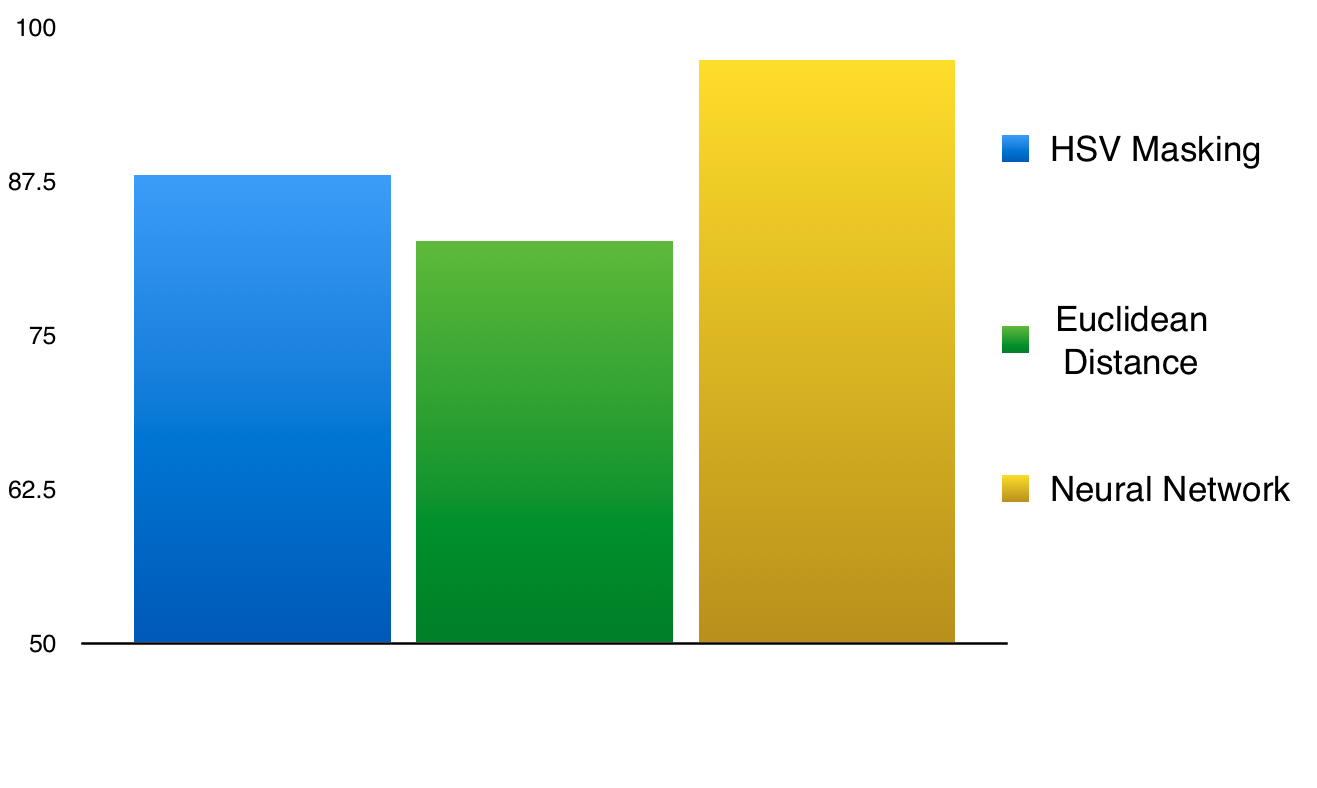
\includegraphics[width=\textwidth, height=5cm]{colourefficiency.png}
        \label{fig:colefficiency}
    \end{subfigure}
    \begin{subfigure}[H]{0.475\textwidth}   
        \centering 
        \caption{}
        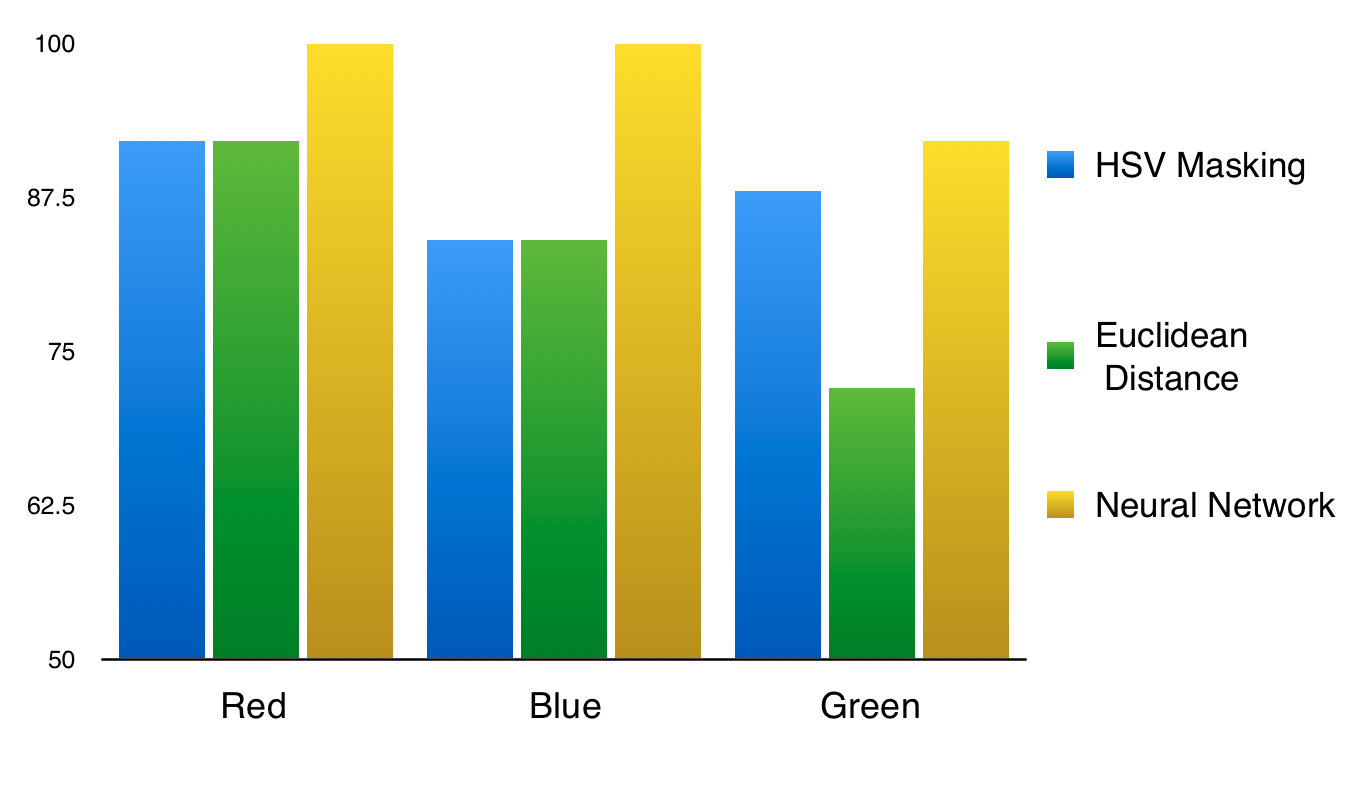
\includegraphics[width=\textwidth, height=5cm]{RGBtesting.png}
        \label{fig:rgbtests}
    \end{subfigure}
    \vspace{-0.5cm}
    \caption{Graphs for colour detection methods: (a) Percentage efficiency of colour detection across multiple methods. (b) Percentage efficiency of RGB detection across multiple methods.}
\end{figure}
As you can see from the RGB tests in \textbf{\Cref{fig:rgbtests}}, the green and blue sweets were more difficult to identify than the red sweets. This is because there was a larger overlap in their colourspace. As you can see from the correctly identified sweets previously in \textbf{\Cref{fig:workingneural}}, some of the green sweets definitely have a dark blue-ish tint to them, so it is even difficult for a human to recognise the correct colour. However, from using a large sample of data to train the neural network, the neural network does seem to do a reasonable job of differentiating between the two. It is clearly shown that the neural network not only has the largest percentage efficiency of colour recognition overall (\textbf{\Cref{fig:colefficiency}}), but it was the most efficient at recognising the different colours as well. This is why it was decided that the neural network was the best colour detection method to use overall.
\newline\newline
\textbf{Limitations}\newline
Whilst the neural network did provide an efficient solution to recognising the sweet's colours, the problem was that this technique was only applicable to a specific brand of sweet with unique blue, green and red coloured wrappers. If any other colours or makes of sweet were used, a new training set would have to be created and trained before they could be recognised. A suggestion to solve this would be to create a user interface to allow the user to add their own coloured sweet by taking a sufficient number of photos. The lack of time towards the end of the project meant I did not have time to implement this. Another issue still arose when the colourspaces overlapped too much. For example, the neural network couldn't correctly train itself to tell the difference between pink and red sweets in different lights. To solve this, a more complex network could be developed to allow extra hidden layers for a more robust method for recognising complex colour separations.
\subsection{Manipulation}
\captionsetup[figure]{justification=centering}
\begin{figure}[H]
        \centering 
        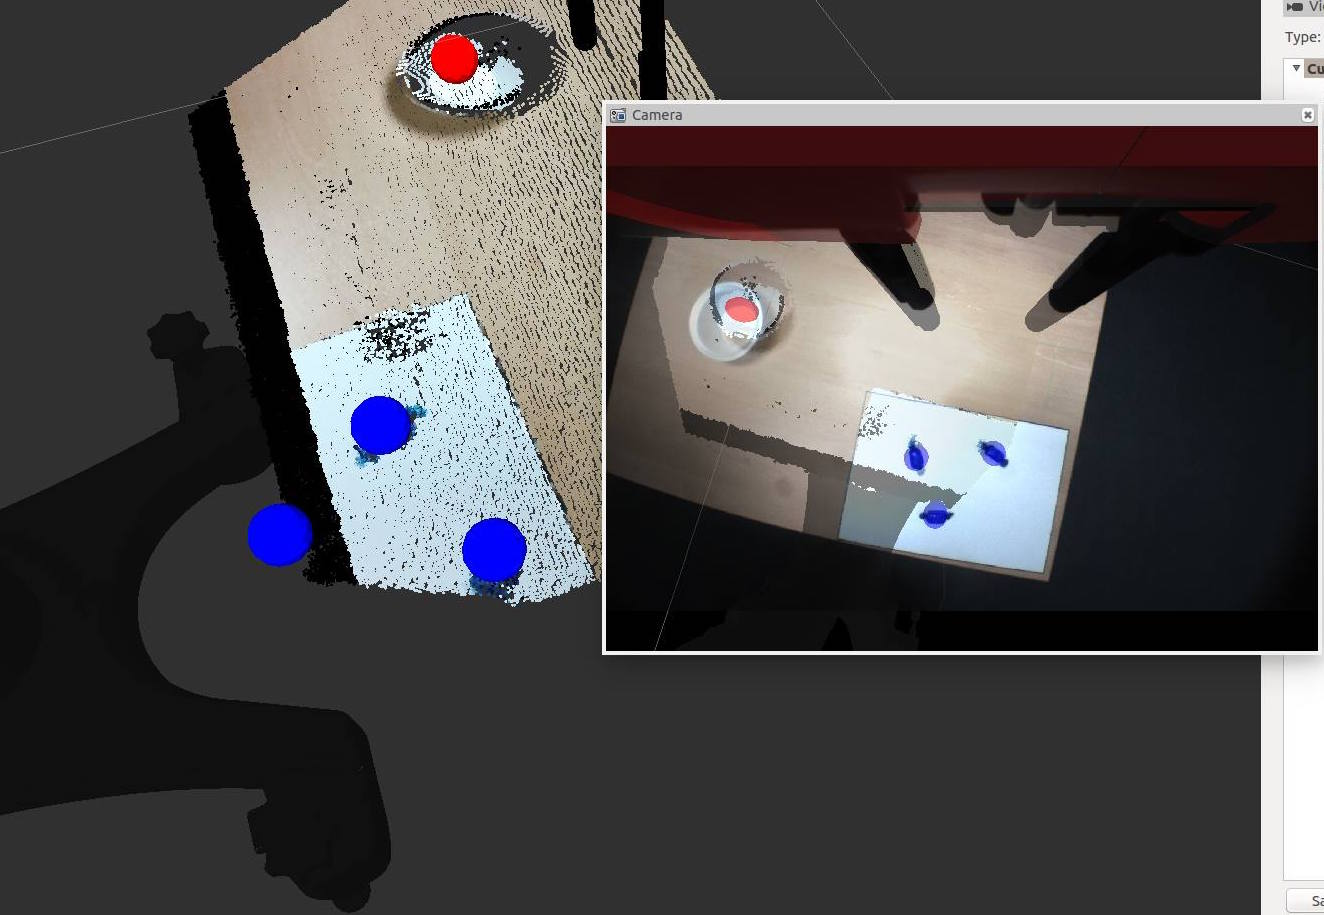
\includegraphics[width=0.475\textwidth, height=5cm]{sweettransformation.jpg}
        \caption{RViz showing the transformation between the detected sweet centres and the actual coordinates.}
        \label{fig:transformationsweets}
\end{figure}
Now there was a method for the sweets to be detected, by extracting moments from the sweet contours, the 2D pixel coordinate could be retrieved from the 2D image. The problem then was converting the 2D points in that image into 3D world coordinates. This was done using an altered version of a pinhole camera method\footnote{OpenCV - Camera calibration and 3D Reconstruction. \url{http://docs.opencv.org/2.4/modules/calib3d/doc/camera\_calibration\_and\_3d\_reconstruction.html}}, where the u, v coordinate within the 2D image could be converted to a 3D world coordinate using Baxter's in-built calibrated camera matrix. The equation uses the x and y camera offset values, with the focal lengths to scale the initial point. Then using the distance from the camera to the table (which is fixed), the points were then converted into 3D world coordinates. This was tested using rViz and Baxter to make sure it worked, shown above in \textbf{\Cref{fig:transformationsweets}}. This method was a difficult concept to grasp, but after some sound mathematical theory in deducing the correct formula, I was pleasantly surprised at how efficient the transformation was.
\subsubsection{Grabbing Methods}
\textbf{Basic Grasp}\newline
Once the sweet positions were known to Baxter, a basic grabbing method was developed initially. This was done by creating a function where the xyz coordinate was known for the centre of the sweet, then Baxter would move his hand directly above the sweet at the default horizontal gripper rotation. Then Baxter slowly moves his hand down and closes his gripper when he reaches the height of the table. This was a very simple approach to grasping sweets that, whilst reasonably reliable, when the sweet's orientation was at an awkward angle, the lack of rotation would cause the sweet to slip out of the gripper on grasping.\newline\newline
\textbf{Grasp with Rotation}
\begin{figure}[H]
    \captionsetup[subfigure]{justification=centering}
    \begin{subfigure}[H]{0.475\textwidth}   
        \centering 
        \caption{}
        \label{fig:PCA}
        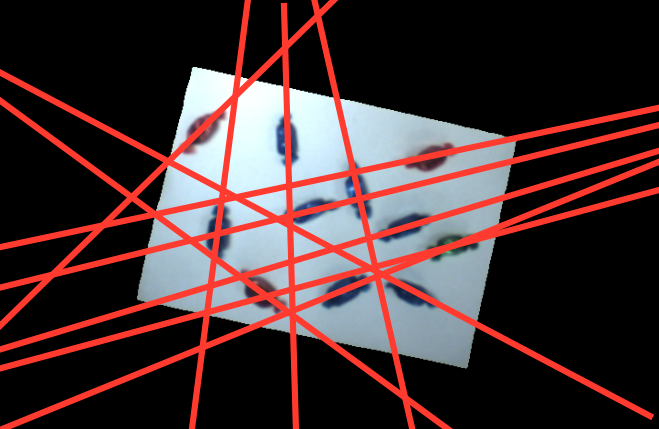
\includegraphics[width=\textwidth, height=5cm]{pcaexample.png}
    \end{subfigure}
    \begin{subfigure}[H]{0.475\textwidth}   
        \centering 
        \caption{}
        \label{fig:RotationGrasp}
        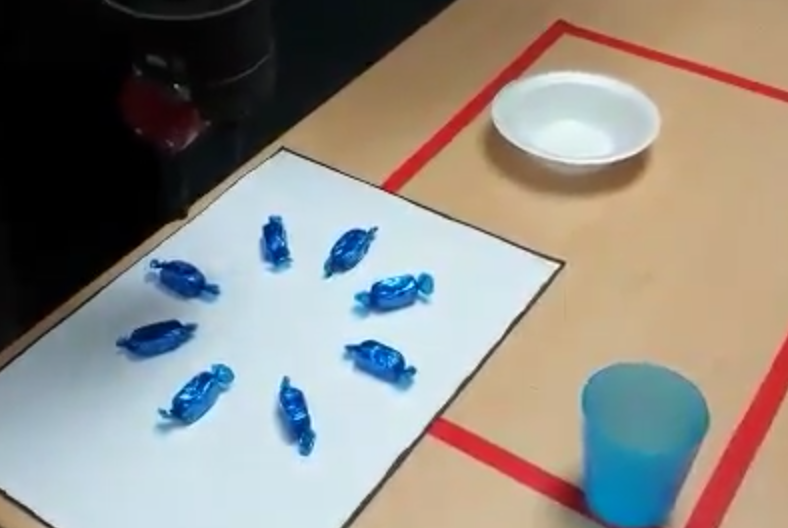
\includegraphics[width=\textwidth, height=5cm]{graspwithrotation.png}
    \end{subfigure}
    \caption{Grasping sweets with rotation: (a) Principle axes of each sweet on the page. (b) An image showing Baxter grasping sweets placed at multiple angles.}
\end{figure}
This grasp used a very similar approach to the previous grasp however, it contained a very important update, it included the rotation of Baxter's gripper. This however, meant that an improvement on the sweet's vision system was needed to work out the angles the sweets were placed at. To do this, a PCA (principal component analysis), was calculated on the contour for each sweet. After the principal axis was calculated for each sweet (shown in \textbf{\Cref{fig:PCA}}), the grippers could be placed perpendicular to that axis to grab the sweets at the correct rotation. Therefore, after finding those perpendicular lines, the angle could be calculated that the gripper needed to rotate by using the formula below. This formula was used with the perpendicular line values against a the horizontal axis to find out the angle Baxter needed to grasp at related to it's default rotation along that axis.
\newline
\[
    cos\theta = \frac{(x_2 - x_1)\cdot(x_4 - x_3)}{|x_2 - x_1||x_4 - x_3|}
\]
\newline
Here, x1 and x2 are the endpoints of the calculated line and x3 and x4 are endpoints of a horizontal line representing the x axis. After calculating the angles, they were sent along with the sweet coordinates so Baxter could know the angle required to pick up each sweet. Once this grasp was working, the pick up efficiency of the sweets became a lot higher and Baxter could grasp sweets at all angles, shown in \textbf{\Cref{fig:RotationGrasp}}. A comparison between the basic and rotation grasping techniques can be seen using the videos on the Github repository\footnote{Github repository: Videos - Sweet Grasping Methods. \url{https://github.com/um10kh/baxter-project/tree/master/videos/Sweet\%20Grasping\%20Methods}}.
\newline\newline
\textbf{Improvements}\newline
Whilst the grasp with rotation method was very efficient at picking up sweets, it did sometimes only grab a small edge of the sweet, then the sweet would slip slowly out of the gripper and fall onto the table. After, Baxter would try and put nothing into the bag, assuming it had grabbed a sweet. The problem with this was Baxter thought he had grabbed a sweet there, whereas ideally, it would've been nice for Baxter to know when he missed a grasp or not. This lead to an alteration using torque-based sweet detection.
\newline\newline
Baxter contains a pressure sensor on the inside of each of his grippers. To detect the pressure, by subscribing to the gripper's state topic, the torque could be retrieved from the gripper at any time. This meant that Baxter could tell whether a sweet was in his hand by detecting whether there was zero torque (no sweet) or some torque (sweet currently in the gripper). By using this technique while Baxter was grasping the sweet, he would know whether or not the sweet was in his gripper. Therefore the improvement was made that he would try and regrasp another sweet if he missed grasping a sweet rather than continuing to put nothing into the sweet container.
\subsubsection{Testing}
To test the grasping methods, they were both measured trying to grasp 10 sweets at various angles from the table (tests found here\footnote{Github repository: Sweet Grasping Tests. \url{https://github.com/um10kh/baxter-project/blob/master/Trials/Sweet\%20Grasping\%20Tests.xlsx}}). To make the tests fair, the sweets were placed in the same orientation for each method. As you can see from \textbf{\Cref{fig:graspTests}}, the variables that were recorded were whether Baxter missed grabbing a sweet completely, whether he partially grasped but dropped the sweet or whether he correctly grabbed the sweet.
\captionsetup[figure]{justification=centering}
\begin{figure}[H]
        \centering 
        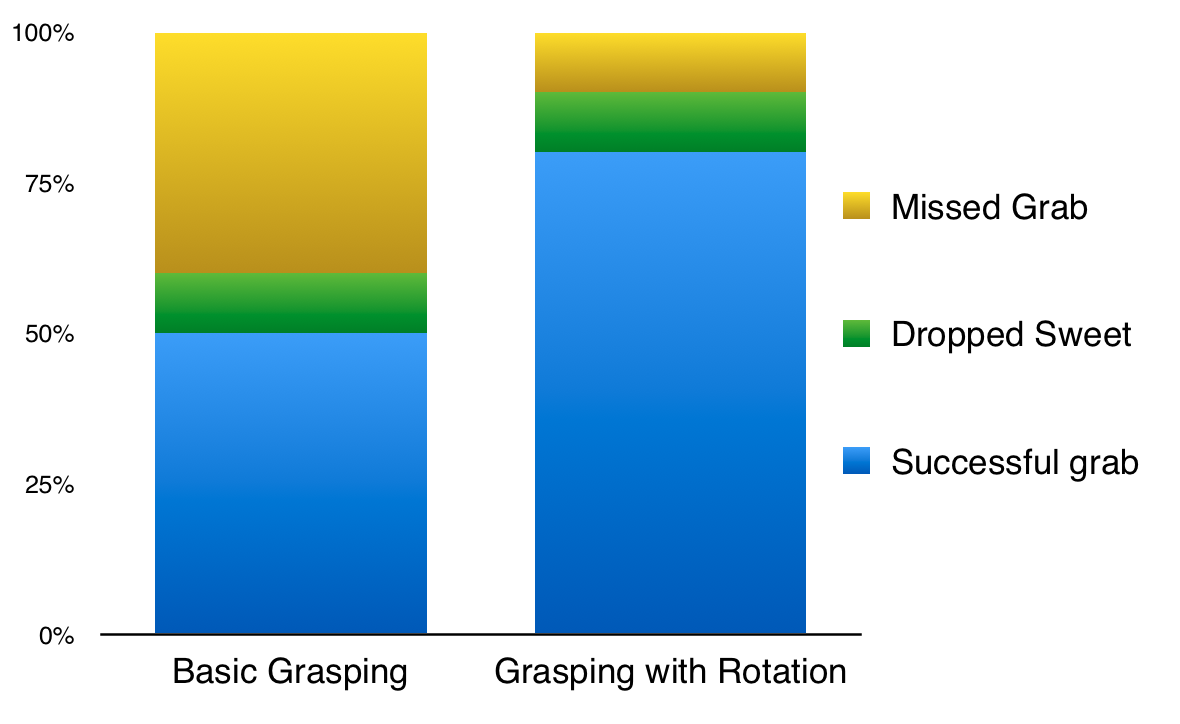
\includegraphics[width=0.475\textwidth, height=5cm]{sweetgrasptests.png}
        \caption{A graph showing the difference in efficiency between the developed sweet grasping techniques.}
        \label{fig:graspTests}
\end{figure}
The graph shows that the grasping with rotation severely reduced the occurrences where Baxter missed the sweets. This showed that adding rotation to the grasping method really increased the efficiency and it was a fairly reliable method to use in the overall system. Some limitations of the approach could be that the approach still misses/drops the occasional sweet. If there was time, the grasping method could be further improved for Baxter to iteratively move towards the sweet and use the vision system to analyse the exact position between the gripper and the target, to make sure it stayed exactly in the centre of the gripper.
\subsection{Singulation}
A major problem with the tipping sweets from the bowl is that it could result in sweets which are too close together to be recognised properly by Baxter's perception system. Without them being properly recognised, Baxter ignores them and therefore can't include them in the overall system. This results in problems say, if the customer wants three red sweets and there are only four in the bowl. If two red sweets are overlapping when tipped onto the table, Baxter could only possibly recognise the other two. This section explains methods used to recognise overlapping sweets and methods to separate them/pick them up from a pile to rectify this problem.
\subsubsection{Detecting Overlaps}
Since the previous sweet recognition system only recognised sweets which were separated from each other on the table via a contour method, large contours of two or more sweets could not be easily recognised. The main problem here was that, due to the sweets not being separable by colour reliably (the colour spaces overlapped), there needed to be a custom vision method developed to separate them. This section discusses the multiple approaches on trying to analyse these larger contours and split them into the respective separate sweets.
\newline\newline
\textbf{Separation by Case}\newline
An initial attempt to split these contours into separate sweets was to code the contour splitting manually by analysing the position, shape and angle of the contours and splitting them the correct way. This method was attempted by first looking at the shape of the contours, the area of them and the ratio between the height and width. 
\captionsetup[figure]{justification=centering}
\begin{figure}[H]
        \centering 
        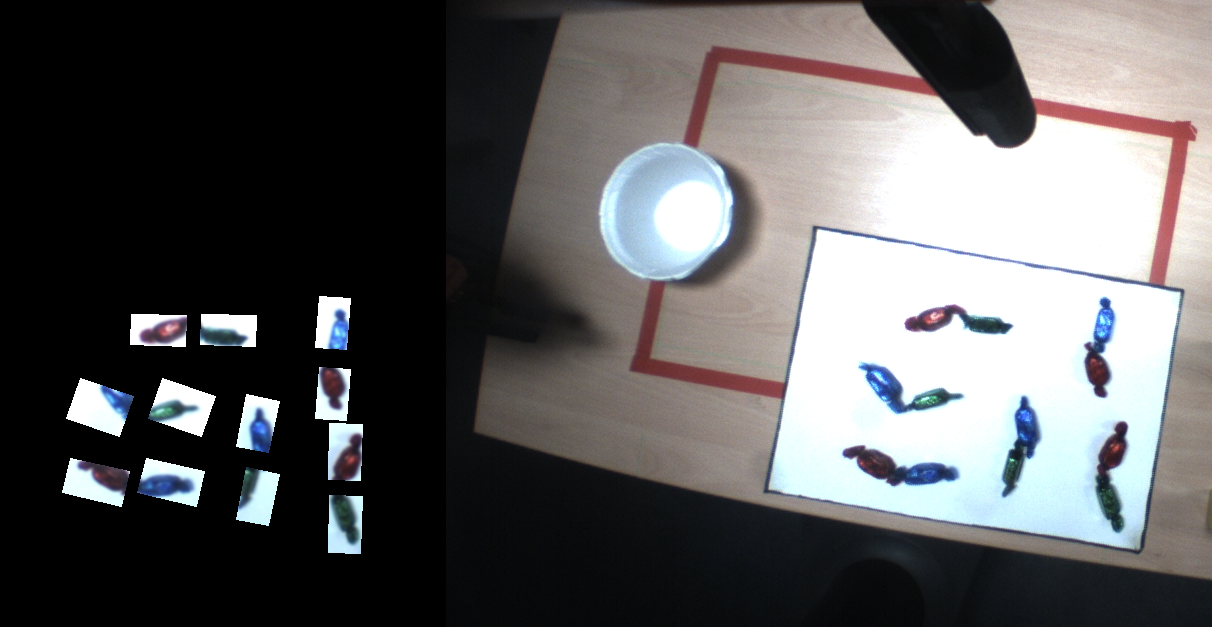
\includegraphics[width=0.7\textwidth, height=5cm]{halvingcollisions.png}
        \caption{An example of splitting contours using a simple case.}
        \label{fig:separatecase}
\end{figure}
Initially, the first case attempted to solve was the one in \textbf{\Cref{fig:separatecase}}, where the sweet contour had a rectangular shape with an area the size of two sweets. As you can see in the image, this case was easily separable and therefore the sweets were recognisable. However, the problem came when attempting to apply this technique to multiple cases. The number of different separable cases were too large and varied to use this technique in practice, so other techniques had to be developed.
\newline\newline
\textbf{Morphological Analysis}\newline
Another attempt to do this was to try and split the sweet contours via morphological analysis. This was done by a few processing methods to dilate and erode the masked sweet images to split them apart into separate elliptical shapes. This approach worked for the most part aside from when two sweets fell next to each other, sharing one of their sides together.
\captionsetup[figure]{justification=centering}
\begin{figure}[H]
        \centering 
        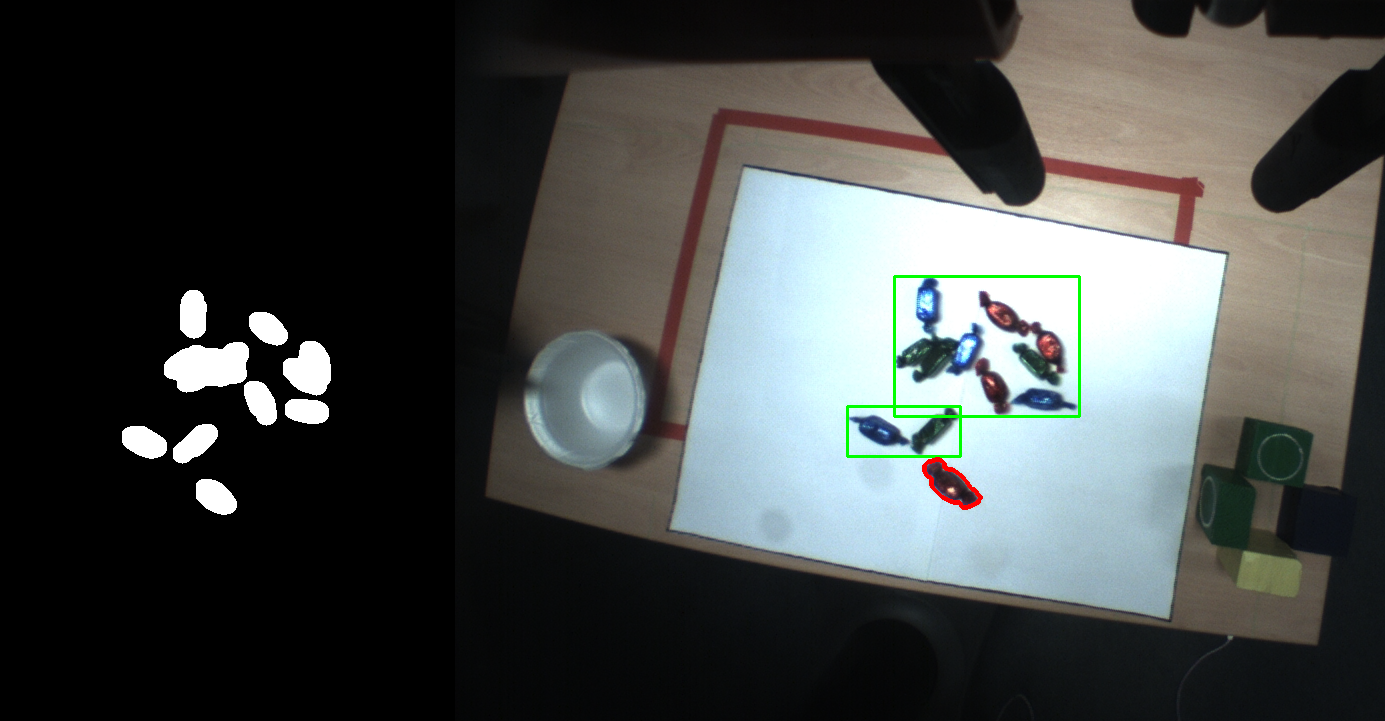
\includegraphics[width=0.7\textwidth, height=5cm]{morphellipse.png}
        \caption{An example of a failed morphological analysis on groups of sweets.}
        \label{fig:morphAnalysis}
\end{figure}
This situation could not be split using this method as the sweets were too close to each other to split via this method. An example of this method failing is shown above in \textbf{\Cref{fig:morphAnalysis}}, where some of the sweets that were very close together couldn't be separated.
\newline\newline
\textbf{Rectangular Search Method}
\newline
The main method used in the final version of the software was the rectangular search method. This method used a combination of vision techniques to process the sweets and separate them within the grouped contour. This process has multiple steps, explained below.
\begin{figure}[H]
    \captionsetup[subfigure]{justification=centering}
    \begin{subfigure}[H]{0.475\textwidth}   
        \centering 
        \caption{}
        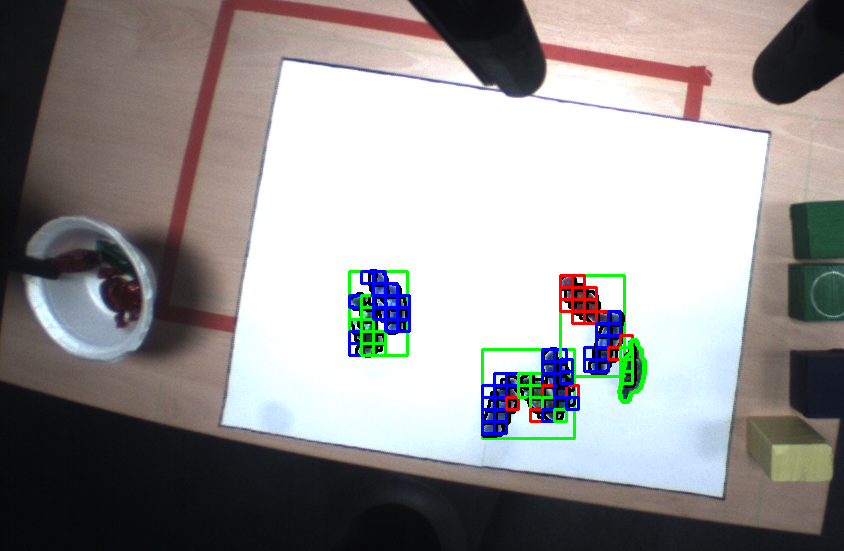
\includegraphics[width=\textwidth, height=5cm]{boxapproach.png}
        \label{fig:boxapproach}
    \end{subfigure}
    \begin{subfigure}[H]{0.475\textwidth}   
        \centering
        \caption{}
        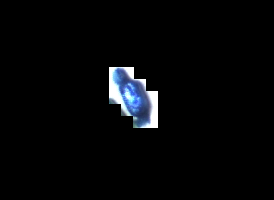
\includegraphics[width=\textwidth, height=5cm]{separatecollisionintoarea.png}
        \label{fig:maskedsweet}
    \end{subfigure}
    \vspace{-0.5cm}
    \caption{Steps for the rectangular search method: (a) Square coloured areas detected within groups of close sweets, (b) A separated sweet mask using the detected blue squares.}
\end{figure}
\textbf{1. Splitting into coloured squares} - Firstly, an algorithm splits the whole contour up into small squares and looks at the colour of each square using the neural network developed in the sweet recognition system. Due to the fact the green, blue and red colourspace has some overlaps in the RGB values, these square colours were not always accurate, but this method was accurate enough to recognise the majority of the sweet's correct colour values (shown in \textbf{\Cref{fig:boxapproach}}).
\newline\newline
\textbf{2. Region Growing Algorithm} - Secondly, a custom region growing algorithm was developed to loop over the coloured squares to grow out the regions. This algorithm checked the horizontal, vertical and diagonal neighbours of each colour and determined the colour was correct if it had two or more of the same neighbours of the same colour. This meant that any anomalous colour recognition, like the anomalous, incorrect colours above, were not included in any further analysis.
\newline\newline
\textbf{3. Masking and Recognition} - After the region growing, the individual sweet areas were converted to a mask, which could then be detected as a whole sweet using the regular image processing techniques normally used in the existing vision system, shown in \textbf{\Cref{fig:maskedsweet}}. 
\begin{figure}[H]
    \captionsetup[subfigure]{justification=centering}
    \begin{subfigure}[H]{0.475\textwidth}   
        \centering 
        \caption{}
        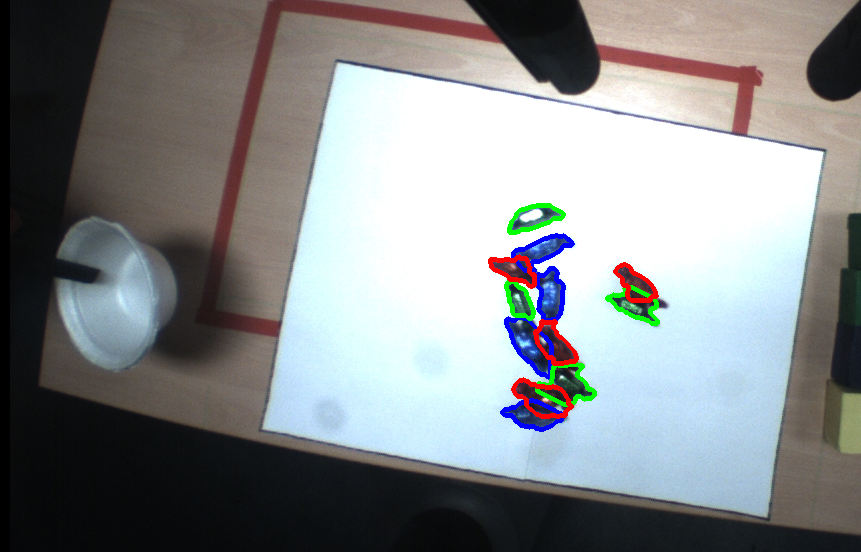
\includegraphics[width=\textwidth, height=5cm]{convexhulloverlappissues.png}
        \label{fig:convexhull}
    \end{subfigure}
    \begin{subfigure}[H]{0.475\textwidth}   
        \centering
        \caption{}
        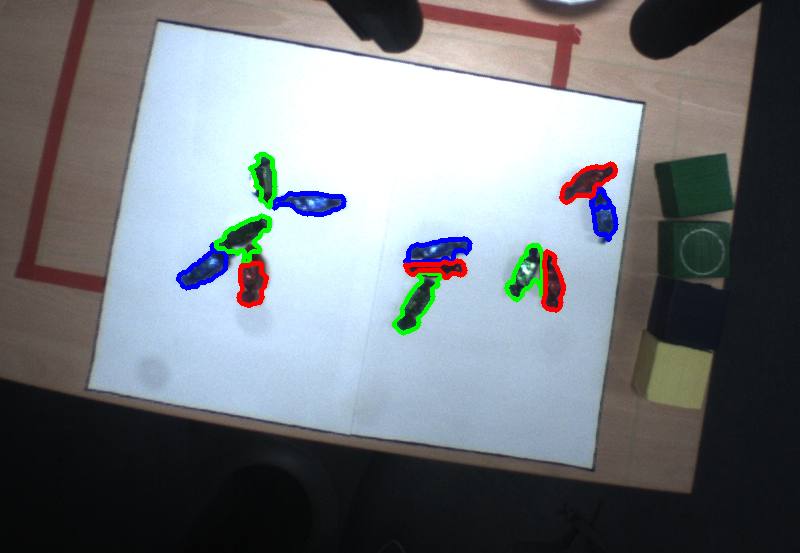
\includegraphics[width=\textwidth, height=5cm]{collisioncorrectdetection.png}
        \label{fig:collisioncorrect}
    \end{subfigure}
    \caption{Detection of overlapping sweets: (a) Sweets detected using convex hulls to expand the detection area. (b) A working example of the vision system detecting overlapping sweets.}
\end{figure}
\textbf{4. Convex Hull/Non Convex Hull Recognition} - Occasionally, the sweet mask missed some of the edges of the sweets, due to the colour edges not being properly recognised. In this case, convex hulls could be taken of the mask, to slightly expand the mask allowing for the whole sweet to be detected. However, convex hulls did have a downside, overlapping the detected sweets as shown in \textbf{\Cref{fig:convexhull}}. It tended to be dependent on the scenario whether the convex hull recognition or non-convex hull recognition was more efficient, so the non-convex hull method was used for the time being, shown in \textbf{\Cref{fig:collisioncorrect}}.
\newline\newline
\textbf{Limitations/Improvements}\newline
Whilst this approach was reasonably efficient, there were some colour detection issues in the earlier stages, leading to slightly inaccurate sweet edge detection. Another limitation on this approach was the speed of this system. This process required multiple steps, multiple loops over areas and the large amounts of time to process and with more time, the process could be more streamlined.
\newline\newline
This process did have issues when sweets of the same colour were next to each other, as they would be recognised as the same contour/sweet. A quick solution was used for this by using a slightly modified version of the separation by case method mentioned before to separate these sweets, provided that there were only two of the same colour sweet touching each other. Since there were only 4 of each colour sweet in the bowl, it was found that three of the same colour sweet touching on the page was not a very common case.
\subsubsection{Singulation Methods}
Once the overlapping sweets had been recognised, Baxter needed a much more accurate manipulation/singulation system to be able to grasp these sweets. When trying to manipulate sweets in a pile, multiple issues were introduced over picking up a singular sweet, such as grabbing two sweets accidentally instead of one or getting the gripper stuck on a nearby sweet, meaning the grippers couldn't reach the table level and close properly.
\newline\newline
\textbf{Gripper Vision System}\newline
Using the detected sweets from the vision system, an approach was proposed where two circles representing the ends of Baxter's electric gripper would be placed either side of a sweet. Then, if those circles didn't collide with a contour of another sweet, then the gripper would in theory be able to go to that location and pick up the sweet. This approach was implemented by doing PCA, similar to the sweet manipulation detection previously. After getting the perpendicular axis to the sweet, the circles representing the ends of the gripper were placed along that axis either side of the sweet as shown in \textbf{\Cref{fig:fakeGripper}}.
\captionsetup[figure]{justification=centering}
\begin{figure}[ht!]
        \centering 
        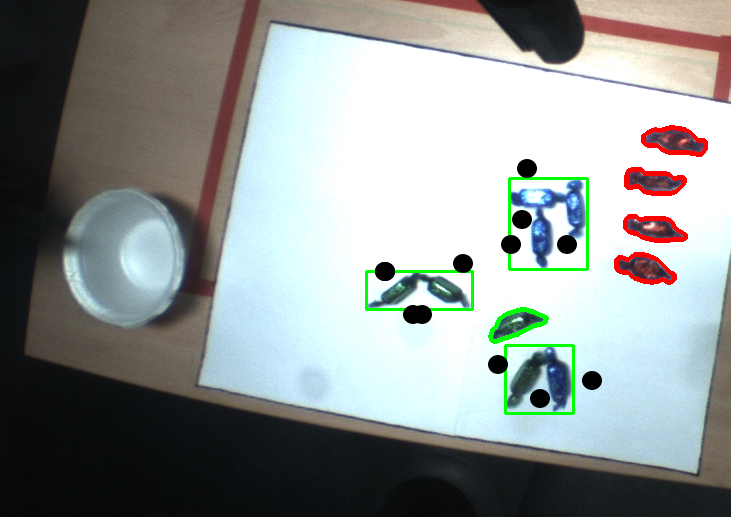
\includegraphics[width=0.475\textwidth, height=5cm]{circlegripperimage.png}
        \caption{An image showing the ends of the gripper projected onto the image where it was possible for Baxter to pick them up.}
         \label{fig:fakeGripper}
\end{figure}
\newline\newline
Then the algorithm checked for collisions of the gripper. If the points for the gripper collided with another sweet contour, then the gripper position would be moved up/down the sweet incrementally to check for an open position. If there was no possible grasping position for the gripper then that sweet was ignored until the pile had been further separated. The idea then was that the vision system would send the respective angles of the sweets that could be separated, Baxter would separate them then re-view the pile to try and grab the other sweets in the next sorted pile. Whilst the theory behind this idea was solid, it was a lot harder to implement the manipulation side of this algorithm (setting custom gripper distances and precise positions caused a lot of issues), so this singulation algorithm was only partially implemented by the end of the project, therefore, definitive testing could not be carried out on this technique.
\section{Human Interaction}
After the main sweet manipulation and recognition methods were initially developed, the final system to implement was human interaction one. Since the human interaction methods were the least important aspect of the overall system (Baxter could get sweets via the command line without any interaction), the human interactions were the least developed at the end of the project, due to time constraints.
\subsection{Voice Recognition}
Voice recognition was a feature that seemed key to implement.within the system. The idea of this feature was for a customer be able to approach Baxter, say a voice command for the requested sweets and then Baxter would get those sweets for them. A couple of approaches were taken to voice recognition, to get the valid accuracy required for an order. The idea was for program to eventually recognise a complex command such as "I would like two green sweets, three blue sweets and one red sweet" and parse the command appropriately.
\subsubsection{Python's NLTK}
Firstly, Python's NLTK module was proposed to be used to analyse voice commands. An in-department microphone was used to record voice commands using some in-built Python microphone recognition/recording modules (the linux alsaaudio module amongst others). This method proved to be difficult to set up and depended on the linux machine and the currently installed drivers. When the microphone installation was set up, a ROS node was created so that the microphone first averaged the background noise to cancel it out. Then the microphone would record until a timed period of speech occurred.
\newline\newline
After the recording was made, the Google API was queried with the audio file, to convert the speech to a line of text. Unfortunately, with noise issues and microphone efficiency issues, there was some difficulty in recognising some words due to the person needing to be a very specific distance from the microphone (otherwise varying noise levels from different distances would interfere with the voice to speech detection). After the speech had been converted to text, the text was analysed to determine the person's command. Since the voice recordings weren't too reliable, the text could be parsed for numbers within the command. The Python module therefore listened three times - for a number for blue, red and green sweets respectively. However, since this didn't recognise full sentences very well, it was decided an Android device could be used to provide a better recording device for more complex, longer commands.
\subsubsection{Android's Google Voice Recognition}
Due to complications with the microphones detecting longer commands, it was decided that an Android device with built-in voice recognition could be a more accurate approach. The only problems with the Android approach is the fact that it assumes an Android device would be available to use alongside Baxter and a small server-client application would have to be developed to run this. Here are some details for the development of this application.
\newline\newline
\textbf{Server-Client Application} 
\newline\newline
\tikzstyle{decision} = [diamond, draw, fill=blue!20, 
    text width=10em, text badly centered, node distance=3cm, inner sep=0pt]
\tikzstyle{block} = [rectangle, draw, fill=blue!20, 
    text width=7em, text centered, rounded corners, minimum height=15em]
\tikzstyle{cloud} = [draw, ellipse,fill=red!20, node distance=3cm,
    maximum height=2em]
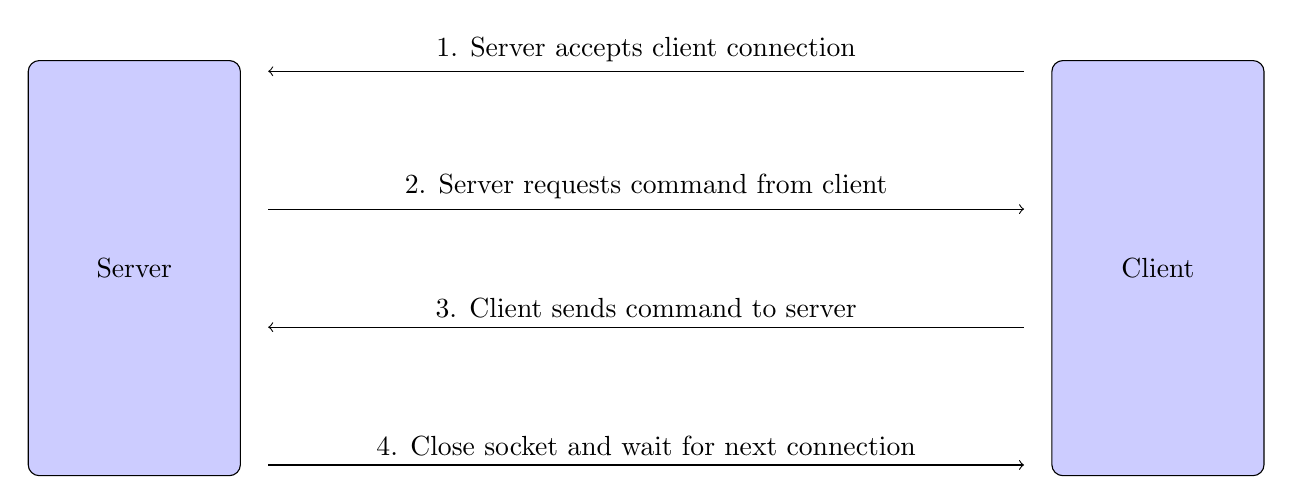
\begin{tikzpicture}[node distance = 2cm, auto]
    % Place nodes
    \node [block] (server){Server};
    \node [block, right of=server] [xshift=11cm] (client) {Client};
    \coordinate (A) at (1.7,0);
    \coordinate (B) at (11.3,0);
    \draw[<-] ([yshift=2.5cm] A) -- ([yshift=2.5cm] B) node [pos=0.5,above] {1. Server accepts client connection};
    \draw[->] ([yshift=0.75cm] A) -- ([yshift=0.75cm] B) node [pos=0.5,above] {2. Server requests  command from client};
    \draw[<-] ([yshift=-0.75cm] A) -- ([yshift=-0.75cm] B) node [pos=0.5,above] {3. Client sends command to server};
    \draw[->] ([yshift=-2.5cm] A) -- ([yshift=-2.5cm] B) node [pos=0.5,above] {4. Close socket and wait for next connection};
\end{tikzpicture}
\newline\newline
The easiest way to connect an Android app with the computer running Baxter's software was to connect a ROS node written in Python to a Java by means of a server-client architecture. The idea being that the Python node would run a server via a Python socket on the university's wireless network and then when a user needs to provide a command, the server would send a command to the client prompting the user to speak or enter a touch command.
\newline\newline
The application client was set up so that it only asks the user for a sweet command when the Python server prompts the client for it. The Python server uses an open '0.0.0.0' IP address on the machine running it and then the client uses the specified wireless IP for the server machine. This is inputted into the app on first opening to ensure that the correct IP address is being used for socket connections between the two devices. The server-client logic is shown above.
\newline\newline
\textbf{User Interface} - The user interface was designed to be simply understood by the user and only require a small amount of setup for the person running the software. The idea of the app is that it would connect to the server on opening, show the main menu and then when Baxter wants a command, the server would send a request to the Java app client, the app would open up the command page, which would prompt the user to record a voice request or enter the sweet numbers they want via touch arrows. The main menu and sweet command page are shown in the images below.
\begin{figure}[H]
    \captionsetup[subfigure]{justification=centering}
    \begin{subfigure}[H]{0.325\textwidth}   
        \centering 
        \caption{}
        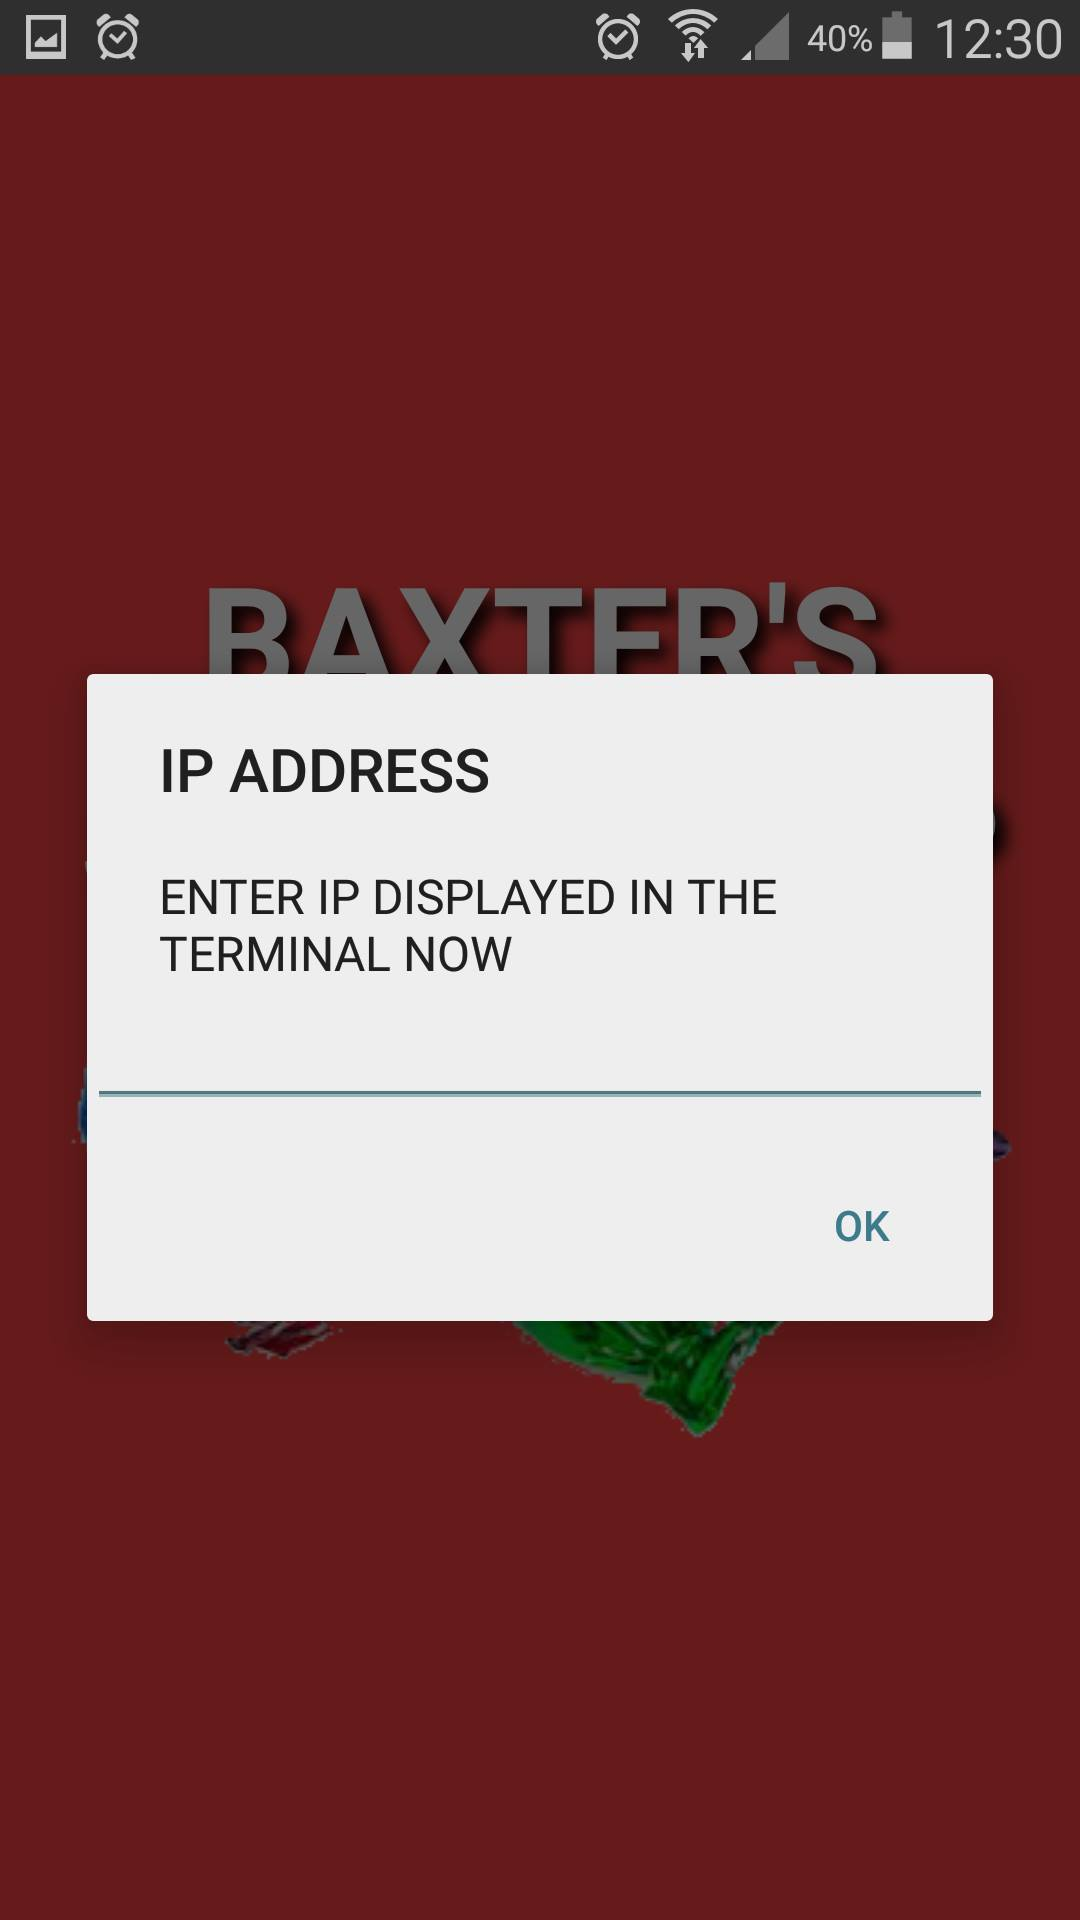
\includegraphics[width=0.8\textwidth, height=7cm]{ipbootpage.png}
        \label{fig:ipEntry}
    \end{subfigure}
    \begin{subfigure}[H]{0.325\textwidth}   
        \centering 
        \caption{}
        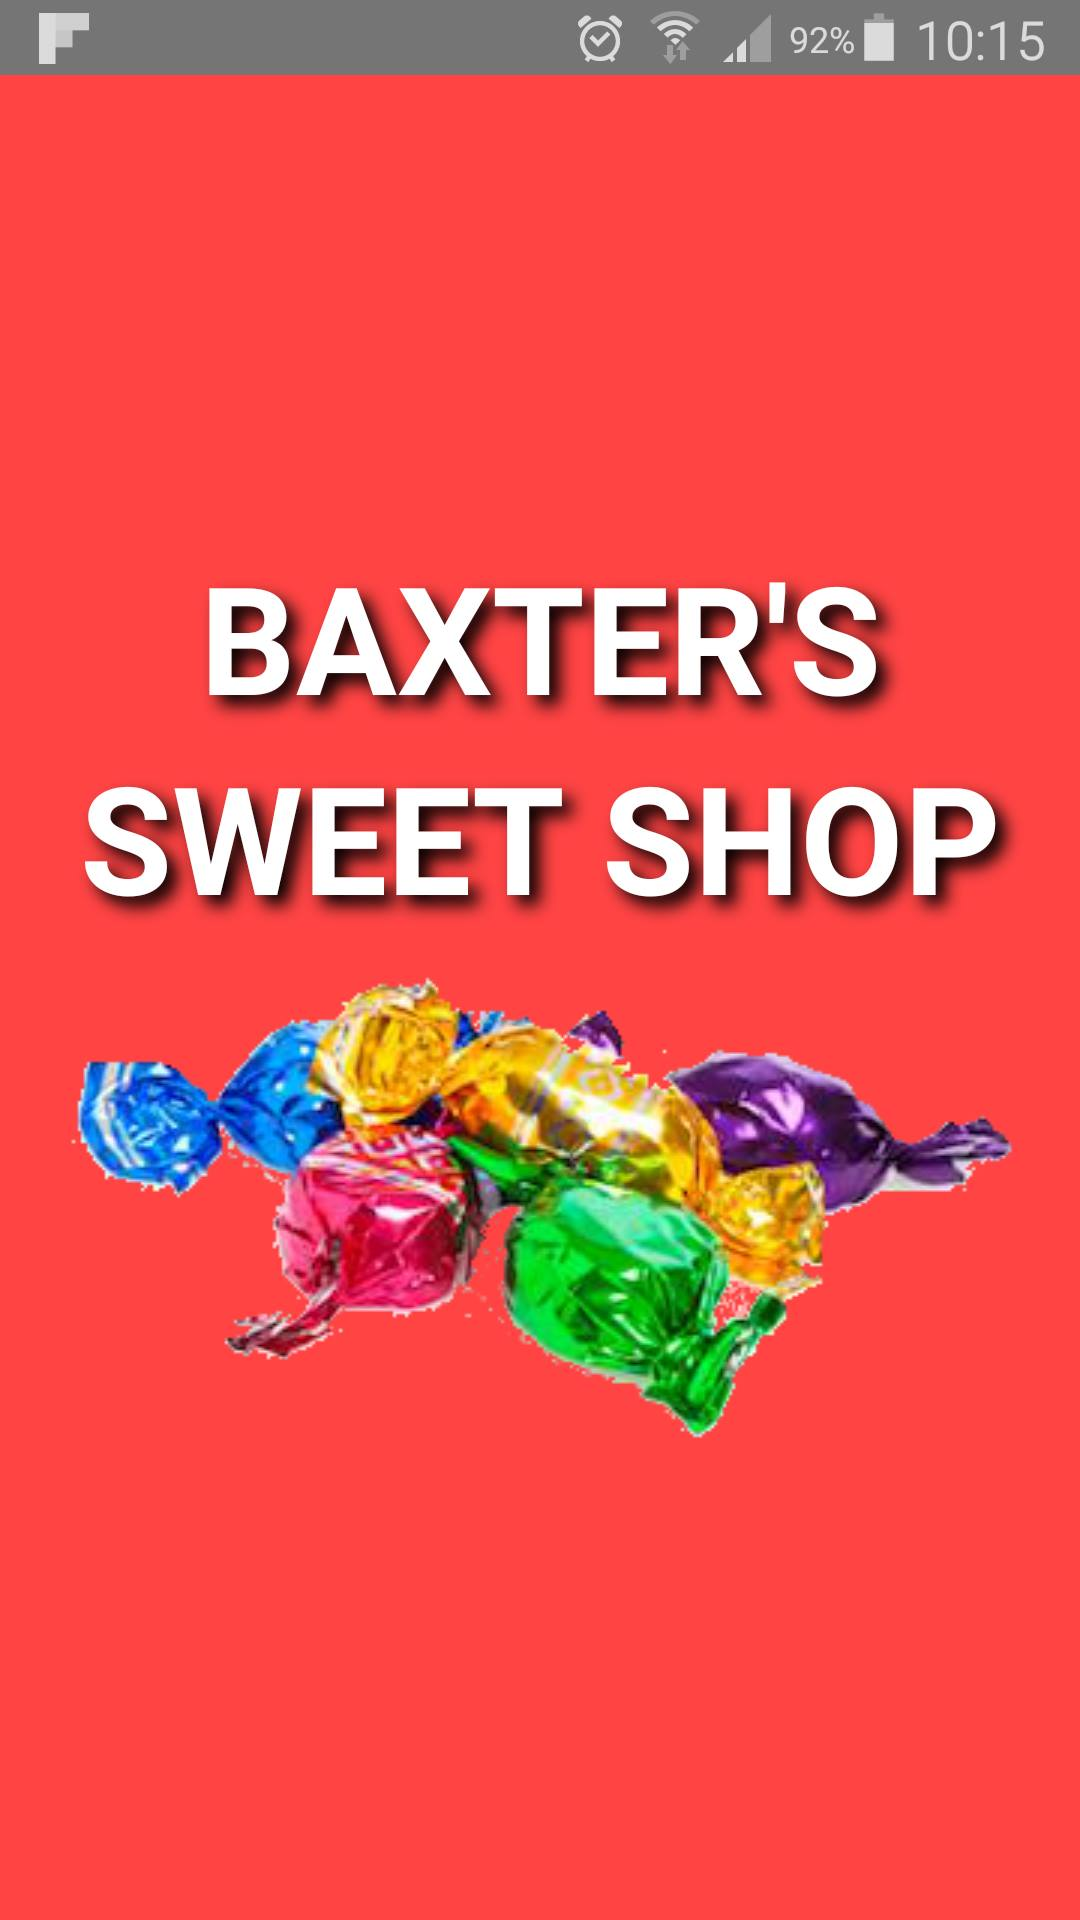
\includegraphics[width=0.8\textwidth, height=7cm]{apphomepage.png}
        \label{fig:appMenu}
    \end{subfigure}
    \begin{subfigure}[H]{0.325\textwidth}   
        \centering 
        \caption{}
        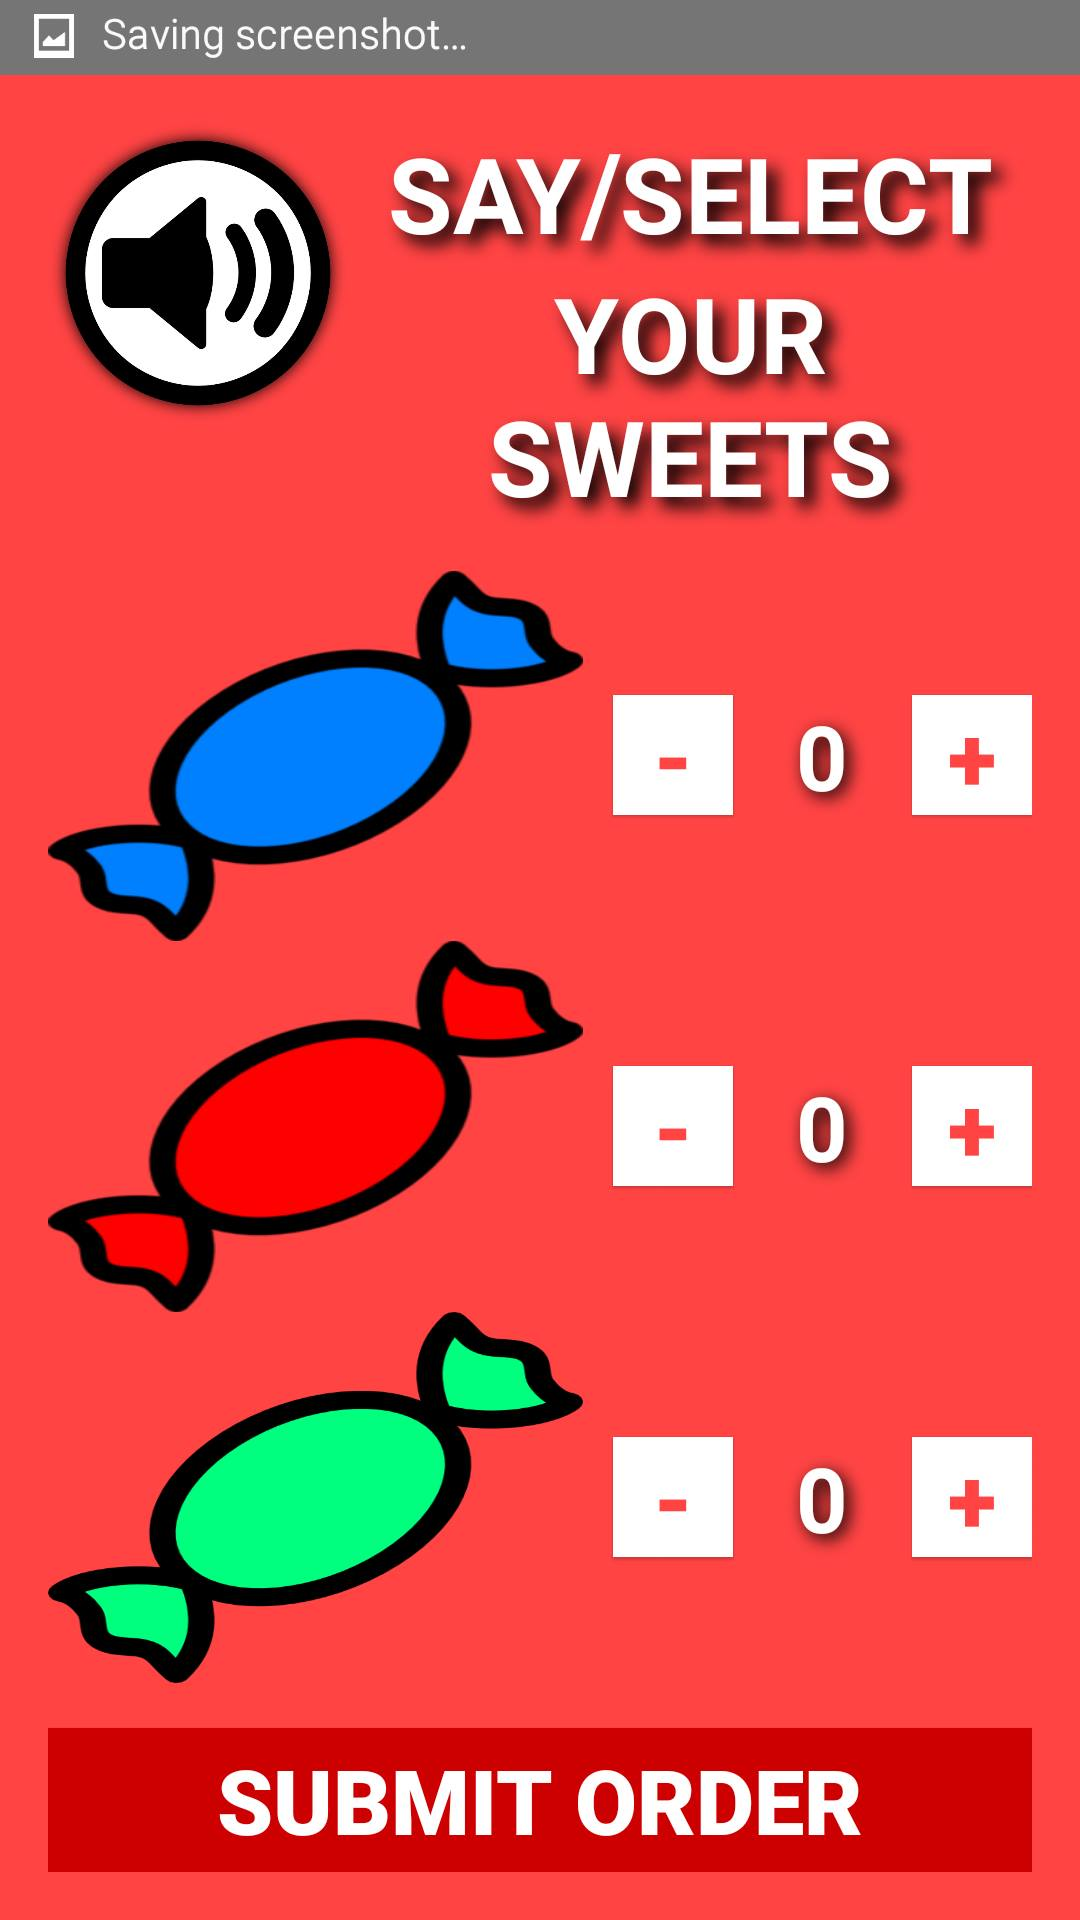
\includegraphics[width=0.8\textwidth, height=7cm]{sweetchoicepage.png}
        \label{fig:appCommand}
    \end{subfigure}
    \caption{Multiple application pages: (a) Enter IP page. (b) Main menu page. (c) Choose sweets page.}
\end{figure}
When the app was opened, the IP address is entered from the command line printed by the server node, entered in \textbf{\Cref{fig:ipEntry}}. Then the main menu page (\textbf{\Cref{fig:appMenu}}) is viewed until the server wants to receive a customer's command, which would go on to the command page (\textbf{\Cref{fig:appCommand}}).
\newline\newline
\textbf{Analyse Command} - After the speech had been converted to text using the Google voice recognition API on the device, the text needed to be parsed for a command. The parsing works in a relatively simple way, where it first looks for whether someone has said the words 'blue', 'green' or 'red'. There is also a basic fuzzy search method where it also looks for other words that sound very similar to them. After, the locations of those words are found and then the words before the colours are analysed, to see what number they are. If they are recognised as 'one', 'two', or 'three', then the parser knows how many of each colour the customer wants. This approach works reliably enough and the more people that tested the system, the more changes and extra anomalies were caught in the voice recognition.
\subsubsection{Testing}
To test the voice recognition approaches using the Python NLTK module and the Android device's voice recognition, firstly, each approach was set up and ten commands were spoken. Each test involved a complex command, which contained a number for blue, red and green sweets for example `Can I have three green, three blue and two red sweets'. The request numbers were varied from one to three and then it was recorded whether all three of the numbers were correctly detected, or whether some were incorrectly recognised.
\captionsetup[figure]{justification=centering}
\begin{figure}[H]
        \centering 
        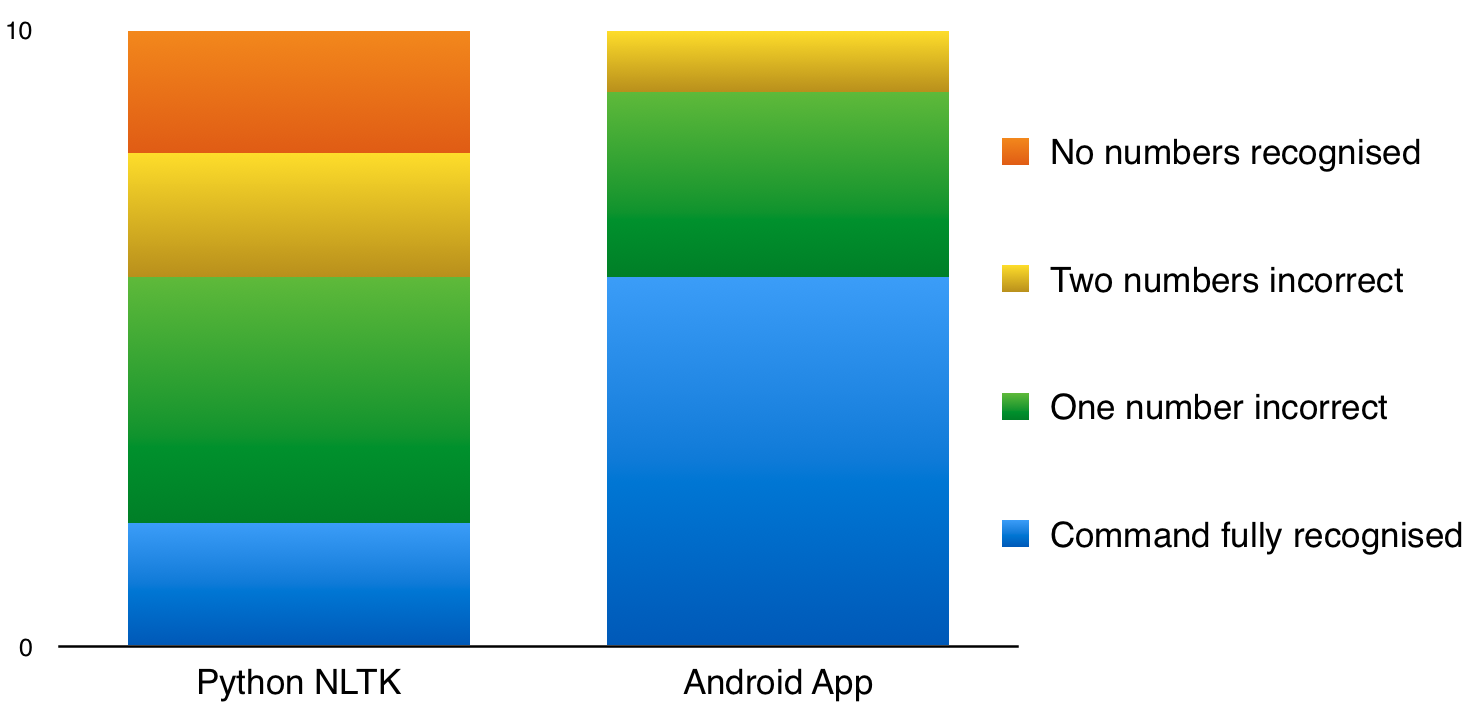
\includegraphics[width=0.6\textwidth, height=5cm]{voicerecognitiontests.png}
        \caption{Voice recognition tests testing the efficiency of the Python NLTK module against the Android voice recognition.}
         \label{fig:voicetests}
\end{figure}
As you can see from \textbf{\Cref{fig:voicetests}}, the android application fully recognised or had one number incorrectly recognised 90\% of the time, as opposed to the python NLTK module, which was far less accurate. This seemed to be due to the noise issues with using a USB microphone rather than a phone microphone. It seemed that varying distance between the customer and a normal microphone seemed to cause a lot more issues with recognition than varying the distance from a phone with the app installed. Therefore, the obvious choice for voice recognition for the overall system was to use the android device.
\subsection{Customer Recognition}
The next implementation of human interaction was to recognise whether a customer has approached Baxter or not. Then if the customer had approached Baxter for some sweets, Baxter would know and could therefore start the conversation and other aspects of the interaction. The initial idea for the approach was to know when a customer enters and exits the scene, to ideally be further expanded to recognise certain actions, like reaching for the sweet bag and exchanging money.
\subsubsection{Detect Person}
The first method to detect a person was a very simply devised method, based around background subtraction without any shape recognition on the person whatsoever. Firstly, Baxter would request a ROS node to look for a person. Then, Baxter would move his arms out of the way so the head could turn and see a customer enter. The current frame would then be used as the background frame for subtraction. A person would be considered to have entered the scene when a large contour was found entering the scene, seen in \textbf{\Cref{fig:personcontour}}. Due to lots of dilation and other pre-processing methods being performed on the image, to make sure the person moving in the scene was recognised as a filled shape, you can see there was some accuracy issues with the contour. However, it was decided that it worked well enough for the basic purpose needed.
\begin{figure}[H]
    \captionsetup[subfigure]{justification=centering}
    \begin{subfigure}[H!]{0.475\textwidth}   
        \centering 
        \caption{}
        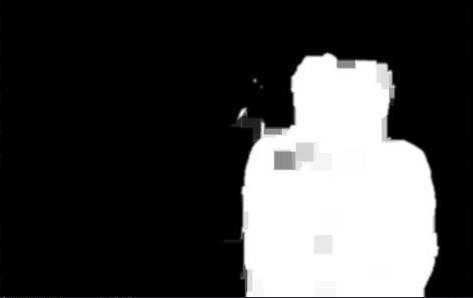
\includegraphics[width=\textwidth, height=5cm]{personprocessing.jpeg}
        \label{fig:TimeGrasp}
    \end{subfigure}
    \begin{subfigure}[H]{0.475\textwidth}   
        \centering 
        \caption{}
        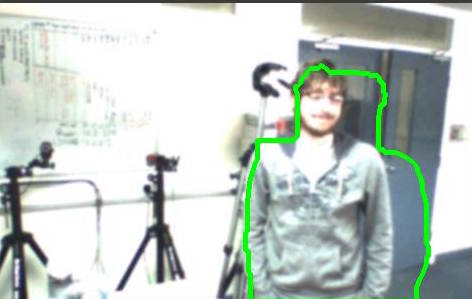
\includegraphics[width=\textwidth, height=5cm]{personrecognised.jpeg}
        \label{fig:personcontour}
    \end{subfigure}
    \vspace{-0.5cm}
    \caption{Person detection methods: (a) Masked person contour differencing from background. (b) Detected person contour in image.}
\end{figure}
After the person was found, a key part of the recognition would be to make sure the person was in front of Baxter for a set period of time. After the person existed in front of the camera for 30 frames, the node recognised the person as wanting sweets and sent a message back to Baxter to start the interaction. However, if a person did not exist for 30 frames, the program would recognise the contour exiting the scene and therefore carry on waiting for another customer.
\newline\newline
This system also had to recognise the opposite feature, when a person left the frame. By keeping the initial background subtracted frame it was possible to find the person contour until it became too small and left off one side of the camera. Then, once the person's contour was not detected anymore, a boolean variable was triggered that allowed Baxter to know that the person had moved away from the camera. This was useful in the process of waiting for one customer leave and another to approach in the shop scenario.
\subsubsection{Skeleton Recognition}
Due to time constraints, a working implementation of skeleton recognition could not be implemented by the end of the project. This was partially due to technological issues. To get a skeleton recognition system working, the system would need to implement a second Kinect depth camera. The problem with a second Kinect is that it was difficult to find a place to put the Kinect, due to one already being on the torso of Baxter looking at the table. This meant the only place to put a second Kinect was on a tripod away from Baxter, meaning that if Baxter was moved at all on open day, that Kinect would have to be recalibrated each time. The decision to not implement skeleton recognition was then made from a time perspective, as it takes a long time to set up an extra Kinect and calibrate it to work with the system. Due to only having 4 weeks left at the point of discussing this, it was decided it was better to focus on other key features of the project.
\subsection{Human Characteristics}
A section that became more important towards the end of the project was adding human-like characteristics to Baxter. With most of the system's features implemented and the human interaction not engaging the customer much, features like giving Baxter a face and a voice added a lot to the overall product.
\subsubsection{Speech System}
For Baxter's speech, a TTS (text-to-speech) module was incorporated to allow Baxter to speak commands and react to certain actions made within the shop. The TTS system used here was the open source module MaryTTS\footnote{The MARY Text-to-Speech System. \url{http://mary.dfki.de/index.html}}. The basic concept of this system is that a Java HTTP server would be hosted, which could convert a client's text request to an output audio file. Whilst there was not an immediately obvious way to translate a Java server/client TTS system to ROS, it helped that a module called \textit{strands\_ui} \footnote{Strands\_ui Github repository. \url{https://github.com/strands-project/strands\_ui}}  existed, which included user interfaces for robots. After installing strands\_ui onto the ros workspace, the server could then be started. Then, a ROS bridge connection was made, allowing a call to me made from the main shopkeeper node to the `ros\_mary\_tts' node, which would then post a HTTP request to the TTS server, get an audio response and send that audio to Baxter.\newline\newline
The TTS system came in handy from translating the shopkeeper program from a mute terminal-based piece of software to a genuine conversation between Baxter and the customer. It helped when Baxter needed to instruct the customer, such as when he needed the customer to speak to place their order, or even just to voice his frustration when he dropped a sweet onto the table.
\subsubsection{Facial Expressions}
Whilst only a small addition to the overall project, different faces were used for Baxter to show different emotions at different interactions in the shop. Multiple images\footnote{Github repository: Baxter's Facial Expressions. \url{https://github.com/um10kh/baxter-project/tree/master/src/manipulation/src/images}} were used to represent a few facial expressions for Baxter. These were mainly to help accentuate the different features of the system and helped in testing to identify what was going on when away from the computer monitor in front of Baxter. A change from a bored default face to a happy face would occur when a customer went in/out of Baxter's sight. A frustrated face would occur when Baxter accidentally dropped a sweet and a happy face would happen at the end of the successful interaction. Small touches like these faces helped to further the human characteristics of Baxter in this interaction, along with adding a little humour as well.